% Options for packages loaded elsewhere
\PassOptionsToPackage{unicode}{hyperref}
\PassOptionsToPackage{hyphens}{url}
%
\documentclass[
  12pt,
]{article}
\usepackage{amsmath,amssymb}
\usepackage{lmodern}
\usepackage{iftex}
\ifPDFTeX
  \usepackage[T1]{fontenc}
  \usepackage[utf8]{inputenc}
  \usepackage{textcomp} % provide euro and other symbols
\else % if luatex or xetex
  \usepackage{unicode-math}
  \defaultfontfeatures{Scale=MatchLowercase}
  \defaultfontfeatures[\rmfamily]{Ligatures=TeX,Scale=1}
  \setmainfont[]{Times New Roman}
\fi
% Use upquote if available, for straight quotes in verbatim environments
\IfFileExists{upquote.sty}{\usepackage{upquote}}{}
\IfFileExists{microtype.sty}{% use microtype if available
  \usepackage[]{microtype}
  \UseMicrotypeSet[protrusion]{basicmath} % disable protrusion for tt fonts
}{}
\makeatletter
\@ifundefined{KOMAClassName}{% if non-KOMA class
  \IfFileExists{parskip.sty}{%
    \usepackage{parskip}
  }{% else
    \setlength{\parindent}{0pt}
    \setlength{\parskip}{6pt plus 2pt minus 1pt}}
}{% if KOMA class
  \KOMAoptions{parskip=half}}
\makeatother
\usepackage{xcolor}
\usepackage[margin=2.54cm]{geometry}
\usepackage{color}
\usepackage{fancyvrb}
\newcommand{\VerbBar}{|}
\newcommand{\VERB}{\Verb[commandchars=\\\{\}]}
\DefineVerbatimEnvironment{Highlighting}{Verbatim}{commandchars=\\\{\}}
% Add ',fontsize=\small' for more characters per line
\usepackage{framed}
\definecolor{shadecolor}{RGB}{248,248,248}
\newenvironment{Shaded}{\begin{snugshade}}{\end{snugshade}}
\newcommand{\AlertTok}[1]{\textcolor[rgb]{0.94,0.16,0.16}{#1}}
\newcommand{\AnnotationTok}[1]{\textcolor[rgb]{0.56,0.35,0.01}{\textbf{\textit{#1}}}}
\newcommand{\AttributeTok}[1]{\textcolor[rgb]{0.77,0.63,0.00}{#1}}
\newcommand{\BaseNTok}[1]{\textcolor[rgb]{0.00,0.00,0.81}{#1}}
\newcommand{\BuiltInTok}[1]{#1}
\newcommand{\CharTok}[1]{\textcolor[rgb]{0.31,0.60,0.02}{#1}}
\newcommand{\CommentTok}[1]{\textcolor[rgb]{0.56,0.35,0.01}{\textit{#1}}}
\newcommand{\CommentVarTok}[1]{\textcolor[rgb]{0.56,0.35,0.01}{\textbf{\textit{#1}}}}
\newcommand{\ConstantTok}[1]{\textcolor[rgb]{0.00,0.00,0.00}{#1}}
\newcommand{\ControlFlowTok}[1]{\textcolor[rgb]{0.13,0.29,0.53}{\textbf{#1}}}
\newcommand{\DataTypeTok}[1]{\textcolor[rgb]{0.13,0.29,0.53}{#1}}
\newcommand{\DecValTok}[1]{\textcolor[rgb]{0.00,0.00,0.81}{#1}}
\newcommand{\DocumentationTok}[1]{\textcolor[rgb]{0.56,0.35,0.01}{\textbf{\textit{#1}}}}
\newcommand{\ErrorTok}[1]{\textcolor[rgb]{0.64,0.00,0.00}{\textbf{#1}}}
\newcommand{\ExtensionTok}[1]{#1}
\newcommand{\FloatTok}[1]{\textcolor[rgb]{0.00,0.00,0.81}{#1}}
\newcommand{\FunctionTok}[1]{\textcolor[rgb]{0.00,0.00,0.00}{#1}}
\newcommand{\ImportTok}[1]{#1}
\newcommand{\InformationTok}[1]{\textcolor[rgb]{0.56,0.35,0.01}{\textbf{\textit{#1}}}}
\newcommand{\KeywordTok}[1]{\textcolor[rgb]{0.13,0.29,0.53}{\textbf{#1}}}
\newcommand{\NormalTok}[1]{#1}
\newcommand{\OperatorTok}[1]{\textcolor[rgb]{0.81,0.36,0.00}{\textbf{#1}}}
\newcommand{\OtherTok}[1]{\textcolor[rgb]{0.56,0.35,0.01}{#1}}
\newcommand{\PreprocessorTok}[1]{\textcolor[rgb]{0.56,0.35,0.01}{\textit{#1}}}
\newcommand{\RegionMarkerTok}[1]{#1}
\newcommand{\SpecialCharTok}[1]{\textcolor[rgb]{0.00,0.00,0.00}{#1}}
\newcommand{\SpecialStringTok}[1]{\textcolor[rgb]{0.31,0.60,0.02}{#1}}
\newcommand{\StringTok}[1]{\textcolor[rgb]{0.31,0.60,0.02}{#1}}
\newcommand{\VariableTok}[1]{\textcolor[rgb]{0.00,0.00,0.00}{#1}}
\newcommand{\VerbatimStringTok}[1]{\textcolor[rgb]{0.31,0.60,0.02}{#1}}
\newcommand{\WarningTok}[1]{\textcolor[rgb]{0.56,0.35,0.01}{\textbf{\textit{#1}}}}
\usepackage{graphicx}
\makeatletter
\def\maxwidth{\ifdim\Gin@nat@width>\linewidth\linewidth\else\Gin@nat@width\fi}
\def\maxheight{\ifdim\Gin@nat@height>\textheight\textheight\else\Gin@nat@height\fi}
\makeatother
% Scale images if necessary, so that they will not overflow the page
% margins by default, and it is still possible to overwrite the defaults
% using explicit options in \includegraphics[width, height, ...]{}
\setkeys{Gin}{width=\maxwidth,height=\maxheight,keepaspectratio}
% Set default figure placement to htbp
\makeatletter
\def\fps@figure{htbp}
\makeatother
\setlength{\emergencystretch}{3em} % prevent overfull lines
\providecommand{\tightlist}{%
  \setlength{\itemsep}{0pt}\setlength{\parskip}{0pt}}
\setcounter{secnumdepth}{5}
\usepackage{booktabs}
\usepackage{longtable}
\usepackage{array}
\usepackage{multirow}
\usepackage{wrapfig}
\usepackage{float}
\usepackage{colortbl}
\usepackage{pdflscape}
\usepackage{tabu}
\usepackage{threeparttable}
\usepackage{threeparttablex}
\usepackage[normalem]{ulem}
\usepackage{makecell}
\usepackage{xcolor}
\ifLuaTeX
  \usepackage{selnolig}  % disable illegal ligatures
\fi
\IfFileExists{bookmark.sty}{\usepackage{bookmark}}{\usepackage{hyperref}}
\IfFileExists{xurl.sty}{\usepackage{xurl}}{} % add URL line breaks if available
\urlstyle{same} % disable monospaced font for URLs
\hypersetup{
  pdftitle={Insert title of project here},
  pdfauthor={Irene Chang, Susanna Jenkins, and Jordan Mullens},
  hidelinks,
  pdfcreator={LaTeX via pandoc}}

\title{Insert title of project here}
\usepackage{etoolbox}
\makeatletter
\providecommand{\subtitle}[1]{% add subtitle to \maketitle
  \apptocmd{\@title}{\par {\large #1 \par}}{}{}
}
\makeatother
\subtitle{\url{https://github.com/mullja21/Mullens_Chang_Jenkins_872_EDA_Final.git}}
\author{Irene Chang, Susanna Jenkins, and Jordan Mullens}
\date{}

\begin{document}
\maketitle

\newpage
\tableofcontents 
\newpage
\listoftables 
\newpage
\listoffigures 
\newpage

\hypertarget{rationale-and-research-questions}{%
\section{Rationale and Research
Questions}\label{rationale-and-research-questions}}

Question 1: Was the year-over-year change in public investment in
lower-carbon energy RD\&D significant during the Obama administration?

\newpage

\hypertarget{dataset-information}{%
\section{Dataset Information}\label{dataset-information}}

The dataset utilized in this analysis was downloaded from International
Energy Agency. The IEA's Energy Technology RD\&D (Research, Development,
\& Demonstration) Budgets database provides spending information by
energy technology in IEA countries from 1974 to 2022. Data is collected
from central or federal government budgets and state-owned companies.
Spending categories encompass renewables, nuclear power, fossil fuels,
hydrogen, fuel cells, and energy efficiency.

\newpage

\hypertarget{data-wrangling}{%
\section{Data Wrangling}\label{data-wrangling}}

Downloaded the Energy Technology RD\&D (Research, Development, \&
Demonstration) Budgets. After importing the data to GitHub and Rstudio,
the raw dataset was wrangled to suit our analysis. A new data frame was
created by extracting the desired years (1985-2015), currency (USD 2021
prices and exchange rates), and economic indications (Total, Fossil
Fuels, and Unallocated) for each country. A variable for year-over-year
percentage (YoY) difference was created to normalize all comparisons.

\begin{Shaded}
\begin{Highlighting}[]
\CommentTok{\#create new data frame, change column names}
\NormalTok{RDD.newcolnames }\OtherTok{\textless{}{-}}\NormalTok{ RDD.raw }\SpecialCharTok{\%\textgreater{}\%}
  \FunctionTok{row\_to\_names}\NormalTok{(}\AttributeTok{row\_number =} \DecValTok{1}\NormalTok{)}

\CommentTok{\#The column names were imported improperly. The first row contains the correct }
\CommentTok{\#column names, so we used the janitor package since they have a function that }
\CommentTok{\#will replace the column names with the first row.}


\NormalTok{RDD.countries }\OtherTok{\textless{}{-}}
  \FunctionTok{filter}\NormalTok{(RDD.newcolnames,}
\NormalTok{         Country }\SpecialCharTok{==} \StringTok{"Germany"} \SpecialCharTok{|}\NormalTok{ Country }\SpecialCharTok{==} \StringTok{"United States"}\NormalTok{,}
\NormalTok{         Currency }\SpecialCharTok{==} \StringTok{"USD (2021 prices and exchange rates)"}\NormalTok{) }\SpecialCharTok{\%\textgreater{}\%}
  \FunctionTok{rename}\NormalTok{(}\StringTok{"Economic.Indicators"} \OtherTok{=} \StringTok{"Economic Indicators"}\NormalTok{)}


\NormalTok{RDD.final }\OtherTok{\textless{}{-}}\NormalTok{ RDD.countries }\SpecialCharTok{\%\textgreater{}\%}
  \FunctionTok{filter}\NormalTok{(Economic.Indicators }\SpecialCharTok{==} \StringTok{"Total Budget"} \SpecialCharTok{|}\NormalTok{ Economic.Indicators }\SpecialCharTok{==} \StringTok{"Unallocated "} \SpecialCharTok{|}\NormalTok{ Economic.Indicators }\SpecialCharTok{==} \StringTok{"Fossil fuels"}\NormalTok{) }\SpecialCharTok{\%\textgreater{}\%}
  \FunctionTok{select}\NormalTok{(}\StringTok{"Country"}\NormalTok{, }\StringTok{"Currency"}\NormalTok{, }\StringTok{"Economic.Indicators"}\NormalTok{, }\StringTok{"1985"}\NormalTok{, }\StringTok{"1986"}\NormalTok{, }\StringTok{"1987"}\NormalTok{, }\StringTok{"1988"}\NormalTok{, }\StringTok{"1989"}\NormalTok{, }\StringTok{"1990"}\NormalTok{, }\StringTok{"1991"}\NormalTok{, }\StringTok{"1992"}\NormalTok{, }\StringTok{"1993"}\NormalTok{, }\StringTok{"1994"}\NormalTok{, }\StringTok{"1995"}\NormalTok{, }\StringTok{"1996"}\NormalTok{, }\StringTok{"1997"}\NormalTok{, }\StringTok{"1998"}\NormalTok{, }\StringTok{"1999"}\NormalTok{, }\StringTok{"2000"}\NormalTok{, }\StringTok{"2001"}\NormalTok{, }\StringTok{"2002"}\NormalTok{, }\StringTok{"2003"}\NormalTok{, }\StringTok{"2004"}\NormalTok{, }\StringTok{"2005"}\NormalTok{, }\StringTok{"2006"}\NormalTok{, }\StringTok{"2007"}\NormalTok{, }\StringTok{"2008"}\NormalTok{, }\StringTok{"2009"}\NormalTok{, }\StringTok{"2010"}\NormalTok{, }\StringTok{"2011"}\NormalTok{, }\StringTok{"2012"}\NormalTok{, }\StringTok{"2013"}\NormalTok{, }\StringTok{"2014"}\NormalTok{, }\StringTok{"2015"}\NormalTok{)}

\NormalTok{RDD.transpose }\OtherTok{\textless{}{-}} \FunctionTok{data.frame}\NormalTok{(}\FunctionTok{t}\NormalTok{(RDD.final))}

\CommentTok{\#In our final data frame, we want each year to have its own row; however, }
\CommentTok{\#in the original dataset, each year was a column. We transposed it.}

\FunctionTok{colnames}\NormalTok{(RDD.transpose) }\OtherTok{\textless{}{-}} \FunctionTok{c}\NormalTok{(}\StringTok{"Germany.FossilFuels"}\NormalTok{, }\StringTok{"Germany.Unallocated"}\NormalTok{, }\StringTok{"Germany.TotalBudget"}\NormalTok{, }\StringTok{"US.FossilFuels"}\NormalTok{, }\StringTok{"US.Unallocated"}\NormalTok{, }\StringTok{"US.TotalBudget"}\NormalTok{)}

\NormalTok{RDD.transpose.rows }\OtherTok{\textless{}{-}}\NormalTok{ RDD.transpose[}\SpecialCharTok{!}\NormalTok{(}\FunctionTok{row.names}\NormalTok{(RDD.transpose) }\SpecialCharTok{\%in\%} \FunctionTok{c}\NormalTok{(}\StringTok{"Country"}\NormalTok{, }\StringTok{"Currency"}\NormalTok{, }\StringTok{"Economic.Indicators"}\NormalTok{)),]}

 
\NormalTok{RDD.transpose.rows }\OtherTok{\textless{}{-}}\NormalTok{ RDD.transpose.rows }\SpecialCharTok{\%\textgreater{}\%}
  \FunctionTok{mutate\_at}\NormalTok{(}\DecValTok{1}\SpecialCharTok{:}\DecValTok{6}\NormalTok{, as.numeric)}

\CommentTok{\#creating frame for US Data}
\NormalTok{RDD.US }\OtherTok{\textless{}{-}} \FunctionTok{data.frame}\NormalTok{(}\AttributeTok{Year=}\FunctionTok{c}\NormalTok{(}\StringTok{"1985"}\NormalTok{, }\StringTok{"1986"}\NormalTok{, }\StringTok{"1987"}\NormalTok{, }\StringTok{"1988"}\NormalTok{, }\StringTok{"1989"}\NormalTok{, }\StringTok{"1990"}\NormalTok{, }\StringTok{"1991"}\NormalTok{, }\StringTok{"1992"}\NormalTok{, }\StringTok{"1993"}\NormalTok{, }\StringTok{"1994"}\NormalTok{, }\StringTok{"1995"}\NormalTok{, }\StringTok{"1996"}\NormalTok{, }\StringTok{"1997"}\NormalTok{, }\StringTok{"1998"}\NormalTok{, }\StringTok{"1999"}\NormalTok{, }\StringTok{"2000"}\NormalTok{, }\StringTok{"2001"}\NormalTok{, }\StringTok{"2002"}\NormalTok{, }\StringTok{"2003"}\NormalTok{, }\StringTok{"2004"}\NormalTok{, }\StringTok{"2005"}\NormalTok{, }\StringTok{"2006"}\NormalTok{, }\StringTok{"2007"}\NormalTok{, }\StringTok{"2008"}\NormalTok{, }\StringTok{"2009"}\NormalTok{, }\StringTok{"2010"}\NormalTok{, }\StringTok{"2011"}\NormalTok{, }\StringTok{"2012"}\NormalTok{, }\StringTok{"2013"}\NormalTok{, }\StringTok{"2014"}\NormalTok{, }\StringTok{"2015"}\NormalTok{), }
                     \AttributeTok{Fossil.Fuel=}\NormalTok{ RDD.transpose.rows}\SpecialCharTok{$}\NormalTok{US.FossilFuels,}
                     \AttributeTok{Unallocated=}\NormalTok{ RDD.transpose.rows}\SpecialCharTok{$}\NormalTok{US.Unallocated,}
                     \AttributeTok{Total.Budget=}\NormalTok{ RDD.transpose.rows}\SpecialCharTok{$}\NormalTok{US.TotalBudget) }\SpecialCharTok{\%\textgreater{}\%}
  \FunctionTok{mutate}\NormalTok{(}\AttributeTok{Low.Carbon.Energy =} \FunctionTok{c}\NormalTok{(Total.Budget}\SpecialCharTok{{-}}\NormalTok{Fossil.Fuel}\SpecialCharTok{{-}}\NormalTok{Unallocated)) }\SpecialCharTok{\%\textgreater{}\%}
  \FunctionTok{mutate}\NormalTok{(}\AttributeTok{Percent.Change =}\NormalTok{ ((Low.Carbon.Energy }\SpecialCharTok{{-}}
                              \FunctionTok{lag}\NormalTok{(Low.Carbon.Energy))}\SpecialCharTok{/}\FunctionTok{lag}\NormalTok{(Low.Carbon.Energy))}\SpecialCharTok{*}\DecValTok{100}\NormalTok{) }\SpecialCharTok{\%\textgreater{}\%}
  \FunctionTok{mutate}\NormalTok{(}\AttributeTok{Country =} \StringTok{"US"}\NormalTok{)}


\CommentTok{\#creating frame for Germany Data}
\NormalTok{RDD.Germany }\OtherTok{\textless{}{-}} \FunctionTok{data.frame}\NormalTok{(}\AttributeTok{Year=}\FunctionTok{c}\NormalTok{(}\StringTok{"1985"}\NormalTok{, }\StringTok{"1986"}\NormalTok{, }\StringTok{"1987"}\NormalTok{, }\StringTok{"1988"}\NormalTok{, }\StringTok{"1989"}\NormalTok{, }\StringTok{"1990"}\NormalTok{, }\StringTok{"1991"}\NormalTok{, }\StringTok{"1992"}\NormalTok{, }\StringTok{"1993"}\NormalTok{, }\StringTok{"1994"}\NormalTok{, }\StringTok{"1995"}\NormalTok{, }\StringTok{"1996"}\NormalTok{, }\StringTok{"1997"}\NormalTok{, }\StringTok{"1998"}\NormalTok{, }\StringTok{"1999"}\NormalTok{, }\StringTok{"2000"}\NormalTok{, }\StringTok{"2001"}\NormalTok{, }\StringTok{"2002"}\NormalTok{, }\StringTok{"2003"}\NormalTok{, }\StringTok{"2004"}\NormalTok{, }\StringTok{"2005"}\NormalTok{, }\StringTok{"2006"}\NormalTok{, }\StringTok{"2007"}\NormalTok{, }\StringTok{"2008"}\NormalTok{, }\StringTok{"2009"}\NormalTok{, }\StringTok{"2010"}\NormalTok{, }\StringTok{"2011"}\NormalTok{, }\StringTok{"2012"}\NormalTok{, }\StringTok{"2013"}\NormalTok{, }\StringTok{"2014"}\NormalTok{, }\StringTok{"2015"}\NormalTok{),}
                          \AttributeTok{Fossil.Fuel=}\NormalTok{ RDD.transpose.rows}\SpecialCharTok{$}\NormalTok{Germany.FossilFuels,}
                          \AttributeTok{Unallocated=}\NormalTok{ RDD.transpose.rows}\SpecialCharTok{$}\NormalTok{Germany.Unallocated,}
                          \AttributeTok{Total.Budget=}\NormalTok{ RDD.transpose.rows}\SpecialCharTok{$}\NormalTok{Germany.TotalBudget) }\SpecialCharTok{\%\textgreater{}\%}
  \FunctionTok{mutate}\NormalTok{(}\AttributeTok{Low.Carbon.Energy =}\NormalTok{ Total.Budget}\SpecialCharTok{{-}}\NormalTok{Fossil.Fuel}\SpecialCharTok{{-}}\NormalTok{Unallocated) }\SpecialCharTok{\%\textgreater{}\%}
  \FunctionTok{mutate}\NormalTok{(}\AttributeTok{Percent.Change =}\NormalTok{ ((Low.Carbon.Energy }\SpecialCharTok{{-}}
                              \FunctionTok{lag}\NormalTok{(Low.Carbon.Energy))}\SpecialCharTok{/}\FunctionTok{lag}\NormalTok{(Low.Carbon.Energy))}\SpecialCharTok{*}\DecValTok{100}\NormalTok{) }\SpecialCharTok{\%\textgreater{}\%}
  \FunctionTok{mutate}\NormalTok{(}\AttributeTok{Country =} \StringTok{"Germany"}\NormalTok{)}
\end{Highlighting}
\end{Shaded}

\begin{Shaded}
\begin{Highlighting}[]
\CommentTok{\#Adding date column to US data frame and transforming it into date object. Also }
\CommentTok{\#adding a column to denote pre or Obama era for graphing.}
\NormalTok{RDD.US.Eras }\OtherTok{\textless{}{-}}\NormalTok{ RDD.US }\SpecialCharTok{\%\textgreater{}\%}
  \FunctionTok{mutate}\NormalTok{(}\AttributeTok{Date =} \FunctionTok{ymd}\NormalTok{(}\FunctionTok{paste0}\NormalTok{(RDD.US}\SpecialCharTok{$}\NormalTok{Year, }\StringTok{"{-}01{-}01"}\NormalTok{))) }\SpecialCharTok{\%\textgreater{}\%}
  \FunctionTok{mutate}\NormalTok{(}\AttributeTok{Era =} \FunctionTok{ifelse}\NormalTok{(Year }\SpecialCharTok{\textless{}=} \DecValTok{2008}\NormalTok{, }\StringTok{"Pre"}\NormalTok{, }\StringTok{"Obama"}\NormalTok{))}

\CommentTok{\#creating one data frame for US and Germany data}
\NormalTok{US.and.Germany.RDD }\OtherTok{\textless{}{-}} \FunctionTok{rbind}\NormalTok{(RDD.Germany, RDD.US)}

\CommentTok{\#Adding Date column to US and Germany dataframe. Formatting so that column is }
\CommentTok{\#transformed to date class}

\NormalTok{US.and.Germany.RDD }\OtherTok{\textless{}{-}}\NormalTok{ US.and.Germany.RDD }\SpecialCharTok{\%\textgreater{}\%}
  \FunctionTok{mutate}\NormalTok{(}\AttributeTok{Date =} \FunctionTok{ymd}\NormalTok{(}\FunctionTok{paste0}\NormalTok{(US.and.Germany.RDD}\SpecialCharTok{$}\NormalTok{Year, }\StringTok{"{-}01{-}01"}\NormalTok{))) }\SpecialCharTok{\%\textgreater{}\%}
  \FunctionTok{mutate}\NormalTok{(}\AttributeTok{Era =} \FunctionTok{ifelse}\NormalTok{(Year }\SpecialCharTok{\textless{}=} \DecValTok{2008}\NormalTok{, }\StringTok{"Pre"}\NormalTok{, }\StringTok{"Obama"}\NormalTok{))}
\end{Highlighting}
\end{Shaded}

\begin{Shaded}
\begin{Highlighting}[]
\CommentTok{\#file for Us and Germany}
\FunctionTok{write.csv}\NormalTok{(US.and.Germany.RDD, }\AttributeTok{row.names =} \ConstantTok{FALSE}\NormalTok{, }\AttributeTok{file =} \StringTok{"./Processed\_Data/US.and.Germany.RDD.csv"}\NormalTok{)}

\CommentTok{\#File for US alone with eras}
\FunctionTok{write.csv}\NormalTok{(RDD.US.Eras, }\AttributeTok{row.names =} \ConstantTok{FALSE}\NormalTok{, }\AttributeTok{file =} \StringTok{"./Processed\_Data/US.Eras.RDD.csv"}\NormalTok{)}
\end{Highlighting}
\end{Shaded}

\newpage

\hypertarget{exploratory-analysis}{%
\section{Exploratory Analysis}\label{exploratory-analysis}}

\begin{Shaded}
\begin{Highlighting}[]
\CommentTok{\#US Data Set}
\FunctionTok{dim}\NormalTok{(RDD.US.Eras)}
\end{Highlighting}
\end{Shaded}

\begin{verbatim}
## [1] 31  9
\end{verbatim}

\begin{Shaded}
\begin{Highlighting}[]
\FunctionTok{colnames}\NormalTok{(RDD.US.Eras)}
\end{Highlighting}
\end{Shaded}

\begin{verbatim}
## [1] "Year"              "Fossil.Fuel"       "Unallocated"      
## [4] "Total.Budget"      "Low.Carbon.Energy" "Percent.Change"   
## [7] "Country"           "Date"              "Era"
\end{verbatim}

\begin{Shaded}
\begin{Highlighting}[]
\FunctionTok{head}\NormalTok{(RDD.US.Eras)}
\end{Highlighting}
\end{Shaded}

\begin{Shaded}
\begin{Highlighting}[]
\CommentTok{\#US and Germany}
\FunctionTok{dim}\NormalTok{(US.and.Germany.RDD)}
\end{Highlighting}
\end{Shaded}

\begin{verbatim}
## [1] 62  9
\end{verbatim}

\begin{Shaded}
\begin{Highlighting}[]
\FunctionTok{colnames}\NormalTok{(US.and.Germany.RDD)}
\end{Highlighting}
\end{Shaded}

\begin{verbatim}
## [1] "Year"              "Fossil.Fuel"       "Unallocated"      
## [4] "Total.Budget"      "Low.Carbon.Energy" "Percent.Change"   
## [7] "Country"           "Date"              "Era"
\end{verbatim}

\begin{Shaded}
\begin{Highlighting}[]
\FunctionTok{head}\NormalTok{(US.and.Germany.RDD)}
\end{Highlighting}
\end{Shaded}

\begin{Shaded}
\begin{Highlighting}[]
\CommentTok{\#creating Germany Data summary}
\NormalTok{Germ.summary }\OtherTok{\textless{}{-}}\NormalTok{ US.and.Germany.RDD }\SpecialCharTok{\%\textgreater{}\%}
  \FunctionTok{filter}\NormalTok{(Country}\SpecialCharTok{==} \StringTok{"Germany"}\NormalTok{) }\SpecialCharTok{\%\textgreater{}\%}
  \FunctionTok{select}\NormalTok{(Fossil.Fuel, Low.Carbon.Energy, Total.Budget, Percent.Change) }\SpecialCharTok{\%\textgreater{}\%}
  \FunctionTok{summary}\NormalTok{()}

\FunctionTok{kable}\NormalTok{(Germ.summary, }\AttributeTok{caption =} \StringTok{"Summary Statistics for Germany"}\NormalTok{)}
\end{Highlighting}
\end{Shaded}

\begin{table}

\caption{\label{tab:calculating the summary statistics for US and Germany and creating tables}Summary Statistics for Germany}
\centering
\begin{tabular}[t]{l|l|l|l|l}
\hline
  &  Fossil.Fuel & Low.Carbon.Energy &  Total.Budget & Percent.Change\\
\hline
 & Min.   :  1.968 & Min.   : 284.2 & Min.   : 300.1 & Min.   :-36.4805\\
\hline
 & 1st Qu.: 18.518 & 1st Qu.: 461.5 & 1st Qu.: 481.2 & 1st Qu.:-10.2964\\
\hline
 & Median : 38.642 & Median : 586.7 & Median : 639.6 & Median :  0.7250\\
\hline
 & Mean   : 70.604 & Mean   : 703.0 & Mean   : 789.3 & Mean   : -0.4935\\
\hline
 & 3rd Qu.: 61.380 & 3rd Qu.: 860.2 & 3rd Qu.:1003.4 & 3rd Qu.:  7.0978\\
\hline
 & Max.   :299.784 & Max.   :1780.8 & Max.   :2080.6 & Max.   : 46.6672\\
\hline
 & NA & NA & NA & NA's   :1\\
\hline
\end{tabular}
\end{table}

\begin{Shaded}
\begin{Highlighting}[]
\CommentTok{\#creating US Pre Obama summary}
\NormalTok{US.Pre.summary }\OtherTok{\textless{}{-}}\NormalTok{ US.and.Germany.RDD }\SpecialCharTok{\%\textgreater{}\%}
  \FunctionTok{filter}\NormalTok{(Country}\SpecialCharTok{==} \StringTok{"US"}\NormalTok{) }\SpecialCharTok{\%\textgreater{}\%}
  \FunctionTok{filter}\NormalTok{(Era}\SpecialCharTok{==} \StringTok{"Pre"}\NormalTok{) }\SpecialCharTok{\%\textgreater{}\%}
  \FunctionTok{select}\NormalTok{(Fossil.Fuel, Low.Carbon.Energy, Total.Budget, Percent.Change) }\SpecialCharTok{\%\textgreater{}\%}
  \FunctionTok{summary}\NormalTok{()}

\FunctionTok{kable}\NormalTok{(US.Pre.summary, }\AttributeTok{caption =} \StringTok{"Summary Statistics for US pre{-}Obama administration"}\NormalTok{)}
\end{Highlighting}
\end{Shaded}

\begin{table}

\caption{\label{tab:calculating the summary statistics for US and Germany and creating tables}Summary Statistics for US pre-Obama administration}
\centering
\begin{tabular}[t]{l|l|l|l|l}
\hline
  &  Fossil.Fuel & Low.Carbon.Energy &  Total.Budget & Percent.Change\\
\hline
 & Min.   : 262.0 & Min.   :2865 & Min.   :3128 & Min.   :-15.829\\
\hline
 & 1st Qu.: 537.4 & 1st Qu.:3130 & 1st Qu.:3803 & 1st Qu.: -5.289\\
\hline
 & Median : 598.6 & Median :3386 & Median :4120 & Median : -2.426\\
\hline
 & Mean   : 653.4 & Mean   :3500 & Mean   :4153 & Mean   :  0.767\\
\hline
 & 3rd Qu.: 697.9 & 3rd Qu.:3605 & 3rd Qu.:4506 & 3rd Qu.:  6.630\\
\hline
 & Max.   :1603.3 & Max.   :4789 & Max.   :5498 & Max.   : 27.712\\
\hline
 & NA & NA & NA & NA's   :1\\
\hline
\end{tabular}
\end{table}

\begin{Shaded}
\begin{Highlighting}[]
\CommentTok{\#creating Obama admin summary}
\NormalTok{US.Obama.summary }\OtherTok{\textless{}{-}}\NormalTok{ US.and.Germany.RDD }\SpecialCharTok{\%\textgreater{}\%}
  \FunctionTok{filter}\NormalTok{(Country}\SpecialCharTok{==} \StringTok{"US"}\NormalTok{) }\SpecialCharTok{\%\textgreater{}\%}
  \FunctionTok{filter}\NormalTok{(Era}\SpecialCharTok{==} \StringTok{"Obama"}\NormalTok{) }\SpecialCharTok{\%\textgreater{}\%}
  \FunctionTok{select}\NormalTok{(Fossil.Fuel, Low.Carbon.Energy, Total.Budget, Percent.Change) }\SpecialCharTok{\%\textgreater{}\%}
  \FunctionTok{summary}\NormalTok{()}

\FunctionTok{kable}\NormalTok{(US.Obama.summary, }\AttributeTok{caption =} \StringTok{"Summary Statistics for Obama administration"}\NormalTok{)}
\end{Highlighting}
\end{Shaded}

\begin{table}

\caption{\label{tab:calculating the summary statistics for US and Germany and creating tables}Summary Statistics for Obama administration}
\centering
\begin{tabular}[t]{l|l|l|l|l}
\hline
  &  Fossil.Fuel & Low.Carbon.Energy &  Total.Budget & Percent.Change\\
\hline
 & Min.   : 371.6 & Min.   :5303 & Min.   : 5869 & Min.   :-34.043\\
\hline
 & 1st Qu.: 435.7 & 1st Qu.:6438 & 1st Qu.: 6873 & 1st Qu.: -4.974\\
\hline
 & Median : 483.7 & Median :6616 & Median : 7099 & Median : -1.910\\
\hline
 & Mean   :1011.9 & Mean   :6692 & Mean   : 7704 & Mean   :  8.170\\
\hline
 & 3rd Qu.: 587.6 & 3rd Qu.:7006 & 3rd Qu.: 7496 & 3rd Qu.: 17.600\\
\hline
 & Max.   :4181.8 & Max.   :8040 & Max.   :12222 & Max.   : 67.887\\
\hline
\end{tabular}
\end{table}

\begin{Shaded}
\begin{Highlighting}[]
\CommentTok{\#US Line Plot}
\NormalTok{RDD.US.Eras.Line.plot }\OtherTok{\textless{}{-}} \FunctionTok{ggplot}\NormalTok{(RDD.US.Eras, }\FunctionTok{aes}\NormalTok{(}\AttributeTok{x =}\NormalTok{ Date)) }\SpecialCharTok{+}
  \FunctionTok{geom\_line}\NormalTok{(}\FunctionTok{aes}\NormalTok{(}\AttributeTok{y =}\NormalTok{ Total.Budget, }\AttributeTok{color=} \StringTok{"Total.Spending"}\NormalTok{)) }\SpecialCharTok{+}
  \FunctionTok{geom\_line}\NormalTok{(}\FunctionTok{aes}\NormalTok{(}\AttributeTok{y =}\NormalTok{ Fossil.Fuel, }\AttributeTok{color=} \StringTok{"Fossil.Fuels"}\NormalTok{)) }\SpecialCharTok{+}
  \FunctionTok{geom\_line}\NormalTok{(}\FunctionTok{aes}\NormalTok{(}\AttributeTok{y =}\NormalTok{ Low.Carbon.Energy, }\AttributeTok{color=} \StringTok{"Low.Carbon"}\NormalTok{)) }\SpecialCharTok{+}
  \FunctionTok{theme}\NormalTok{(}\AttributeTok{axis.text.x =} \FunctionTok{element\_text}\NormalTok{(}\AttributeTok{angle =} \DecValTok{90}\NormalTok{, }\AttributeTok{vjust =} \FloatTok{0.5}\NormalTok{, }\AttributeTok{hjust=}\DecValTok{1}\NormalTok{, }\AttributeTok{size =} \DecValTok{9}\NormalTok{)) }\SpecialCharTok{+}
  \FunctionTok{scale\_color\_manual}\NormalTok{(}\AttributeTok{name =} \StringTok{"Proportion of }\SpecialCharTok{\textbackslash{}n}\StringTok{ RDD Spending"}\NormalTok{, }\AttributeTok{values=} \FunctionTok{c}\NormalTok{(}
    \StringTok{"Fossil.Fuels"} \OtherTok{=} \StringTok{"midnightblue"}\NormalTok{, }
    \StringTok{"Low.Carbon"} \OtherTok{=} \StringTok{"darkolivegreen3"}\NormalTok{, }
    \StringTok{"Total.Spending"} \OtherTok{=} \StringTok{"sienna3"}\NormalTok{)) }\SpecialCharTok{+}
  \FunctionTok{scale\_x\_date}\NormalTok{(}\AttributeTok{date\_breaks =} \StringTok{"3 years"}\NormalTok{, }\AttributeTok{date\_labels =} \StringTok{"\%Y"}\NormalTok{) }\SpecialCharTok{+}
  \FunctionTok{labs}\NormalTok{(}\AttributeTok{title =} \StringTok{"Proportion of }\SpecialCharTok{\textbackslash{}n}\StringTok{ United States RDD }\SpecialCharTok{\textbackslash{}n}\StringTok{ Spending 1985{-}2015"}\NormalTok{,}
       \AttributeTok{y=}\StringTok{"Amount in USD (2021 }\SpecialCharTok{\textbackslash{}n}\StringTok{ Prices and Exchange Rates)"}\NormalTok{,}
       \AttributeTok{x=}\StringTok{"Year"}\NormalTok{,}
       \AttributeTok{color=} \StringTok{"Legend Title"}\NormalTok{)}

\FunctionTok{print}\NormalTok{(RDD.US.Eras.Line.plot)}
\end{Highlighting}
\end{Shaded}

\begin{figure}
\centering
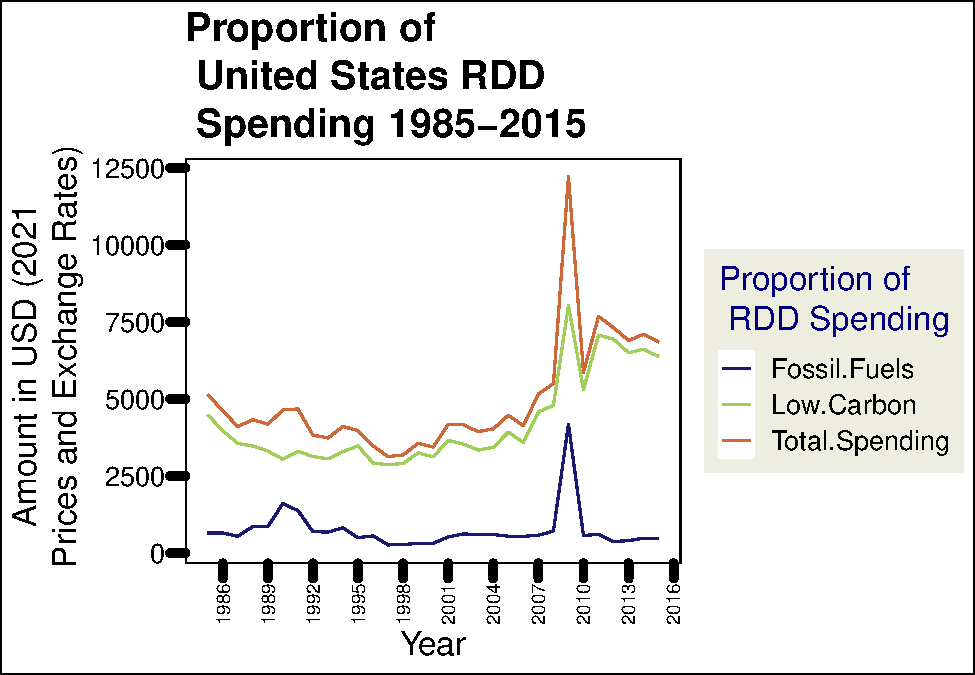
\includegraphics{Chang_Jenkins_Mullens_ENV872_Final_files/figure-latex/Line Plot of All US RDD-1.pdf}
\caption{US RDD Spending 1985 to 2015}
\end{figure}

\begin{Shaded}
\begin{Highlighting}[]
\CommentTok{\# Germ and US Line Plot}
\NormalTok{US.Germ.total.plot }\OtherTok{\textless{}{-}} \FunctionTok{ggplot}\NormalTok{(US.and.Germany.RDD,}
                              \FunctionTok{aes}\NormalTok{(}\AttributeTok{x =}\NormalTok{ Date,}
                                  \AttributeTok{y =}\NormalTok{ Total.Budget, }
                                  \AttributeTok{color =}\NormalTok{ Country)) }\SpecialCharTok{+} 
  \FunctionTok{geom\_line}\NormalTok{(}\AttributeTok{size=} \FloatTok{0.9}\NormalTok{) }\SpecialCharTok{+}
  \FunctionTok{ylim}\NormalTok{(}\DecValTok{0}\NormalTok{, }\DecValTok{12500}\NormalTok{) }\SpecialCharTok{+}
  \FunctionTok{scale\_color\_manual}\NormalTok{(}\AttributeTok{values =} \FunctionTok{c}\NormalTok{(}\StringTok{"tomato3"}\NormalTok{, }\StringTok{"darkblue"}\NormalTok{)) }\SpecialCharTok{+}
  \FunctionTok{labs}\NormalTok{(}\AttributeTok{title =} \StringTok{"Total RDD Spending 1985{-}2015"}\NormalTok{,}
       \AttributeTok{y=}\StringTok{"Amount in USD (2021 }\SpecialCharTok{\textbackslash{}n}\StringTok{ Prices and Exchange Rates)"}\NormalTok{,}
       \AttributeTok{x=}\StringTok{"Year"}\NormalTok{,}
       \AttributeTok{color=} \StringTok{"Legend Title"}\NormalTok{)}
\end{Highlighting}
\end{Shaded}

\begin{verbatim}
## Warning: Using `size` aesthetic for lines was deprecated in ggplot2 3.4.0.
## i Please use `linewidth` instead.
\end{verbatim}

\begin{Shaded}
\begin{Highlighting}[]
\FunctionTok{print}\NormalTok{(US.Germ.total.plot)}
\end{Highlighting}
\end{Shaded}

\begin{figure}
\centering
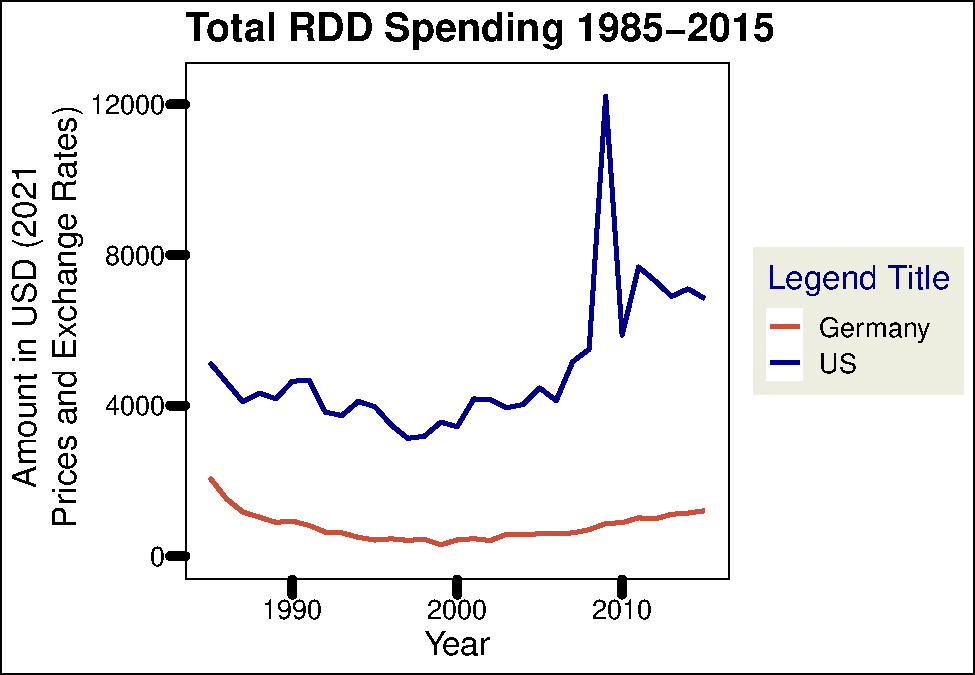
\includegraphics{Chang_Jenkins_Mullens_ENV872_Final_files/figure-latex/Germany and US Line Plot for total budget-1.pdf}
\caption{US and Germany Total RDD Spending 1985 to 2015. Line graph used
to visualize potential trends.}
\end{figure}

\begin{Shaded}
\begin{Highlighting}[]
\CommentTok{\# Create the US and Germ Total bar plot}
\NormalTok{US.Germ.total.Bar.plot }\OtherTok{\textless{}{-}} \FunctionTok{ggplot}\NormalTok{(US.and.Germany.RDD, }\FunctionTok{aes}\NormalTok{(}\AttributeTok{x =}\NormalTok{ Year, }\AttributeTok{y=}\NormalTok{ Total.Budget, }\AttributeTok{fill=}\NormalTok{ Country)) }\SpecialCharTok{+}
  \FunctionTok{geom\_bar}\NormalTok{(}\AttributeTok{stat=} \StringTok{"identity"}\NormalTok{, }\AttributeTok{position =} \StringTok{"stack"}\NormalTok{) }\SpecialCharTok{+}
  \FunctionTok{geom\_bar}\NormalTok{(}\AttributeTok{stat=} \StringTok{"identity"}\NormalTok{, }\AttributeTok{position =} \StringTok{"stack"}\NormalTok{) }\SpecialCharTok{+}
  \FunctionTok{scale\_fill\_manual}\NormalTok{(}\AttributeTok{values =} \FunctionTok{c}\NormalTok{(}\StringTok{"tomato3"}\NormalTok{, }\StringTok{"darkblue"}\NormalTok{)) }\SpecialCharTok{+}
  \FunctionTok{ylim}\NormalTok{(}\DecValTok{0}\NormalTok{, }\DecValTok{15000}\NormalTok{) }\SpecialCharTok{+}
  \FunctionTok{labs}\NormalTok{(}\AttributeTok{fill =} \StringTok{"Country"}\NormalTok{)}\SpecialCharTok{+}
  \FunctionTok{theme}\NormalTok{(}\AttributeTok{axis.text.x =} \FunctionTok{element\_text}\NormalTok{(}\AttributeTok{angle =} \DecValTok{90}\NormalTok{, }\AttributeTok{vjust =} \FloatTok{0.5}\NormalTok{, }\AttributeTok{hjust=}\DecValTok{1}\NormalTok{, }\AttributeTok{size =} \DecValTok{9}\NormalTok{)) }\SpecialCharTok{+}
  \FunctionTok{labs}\NormalTok{(}\AttributeTok{title =} \StringTok{"Total RDD Spending"}\NormalTok{,}
       \AttributeTok{y=}\StringTok{"Amount in USD (2021 }\SpecialCharTok{\textbackslash{}n}\StringTok{ Prices and Exchange Rates)"}\NormalTok{,}
       \AttributeTok{x=}\StringTok{"Year"}\NormalTok{)}
\FunctionTok{print}\NormalTok{(US.Germ.total.Bar.plot)}
\end{Highlighting}
\end{Shaded}

\begin{figure}
\centering
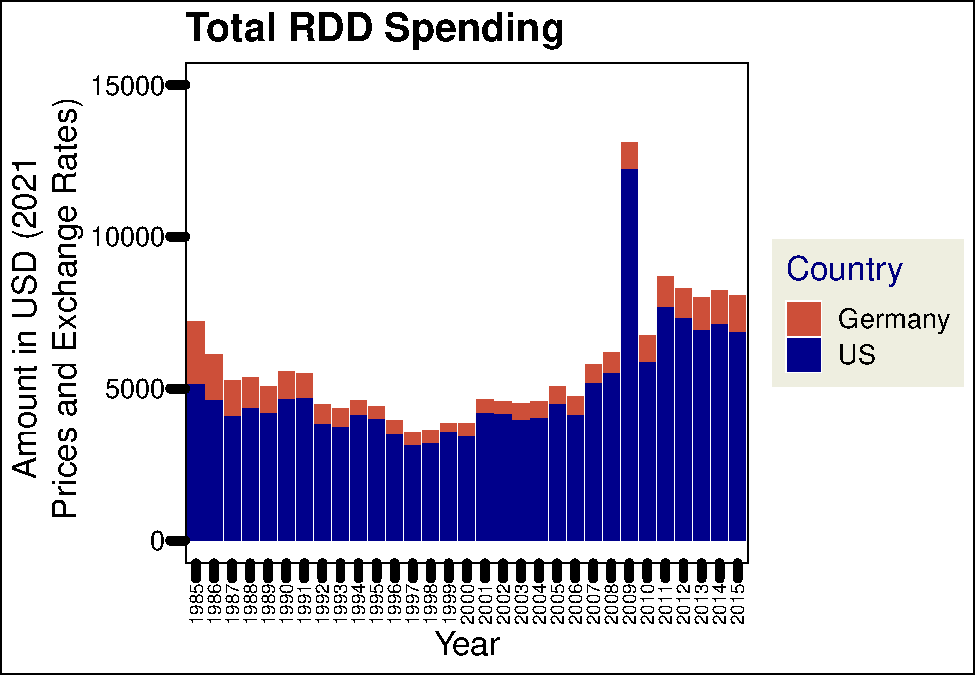
\includegraphics{Chang_Jenkins_Mullens_ENV872_Final_files/figure-latex/Germany and US Bar Plot for total budget-1.pdf}
\caption{US and Germany Total RDD Spending 1985 to 2015. Bar graph used
to visually compare relative magnitude of total spending.}
\end{figure}

\begin{Shaded}
\begin{Highlighting}[]
\CommentTok{\#Fossil Fuel Germ and US Line Plot}
\NormalTok{US.Germ.fossil.plot }\OtherTok{\textless{}{-}} \FunctionTok{ggplot}\NormalTok{(US.and.Germany.RDD,}
                              \FunctionTok{aes}\NormalTok{(}\AttributeTok{x =}\NormalTok{ Date,}
                                  \AttributeTok{y =}\NormalTok{ Fossil.Fuel, }
                                  \AttributeTok{color =}\NormalTok{ Country)) }\SpecialCharTok{+} 
  \FunctionTok{geom\_line}\NormalTok{(}\AttributeTok{size=} \FloatTok{0.9}\NormalTok{) }\SpecialCharTok{+}
  \FunctionTok{ylim}\NormalTok{(}\DecValTok{0}\NormalTok{, }\DecValTok{12500}\NormalTok{) }\SpecialCharTok{+}
  \FunctionTok{scale\_color\_manual}\NormalTok{(}\AttributeTok{values =} \FunctionTok{c}\NormalTok{(}\StringTok{"tomato3"}\NormalTok{, }\StringTok{"darkblue"}\NormalTok{)) }\SpecialCharTok{+}
  \FunctionTok{labs}\NormalTok{(}\AttributeTok{title =} \StringTok{"Fossil Fuel RDD Spending 1985{-}2015"}\NormalTok{,}
       \AttributeTok{y=}\StringTok{"Amount in USD (2021 }\SpecialCharTok{\textbackslash{}n}\StringTok{ Prices and Exchange Rates)"}\NormalTok{,}
       \AttributeTok{x=}\StringTok{"Year"}\NormalTok{,}
       \AttributeTok{color=} \StringTok{"Legend Title"}\NormalTok{)}

\FunctionTok{print}\NormalTok{(US.Germ.fossil.plot)}
\end{Highlighting}
\end{Shaded}

\begin{figure}
\centering
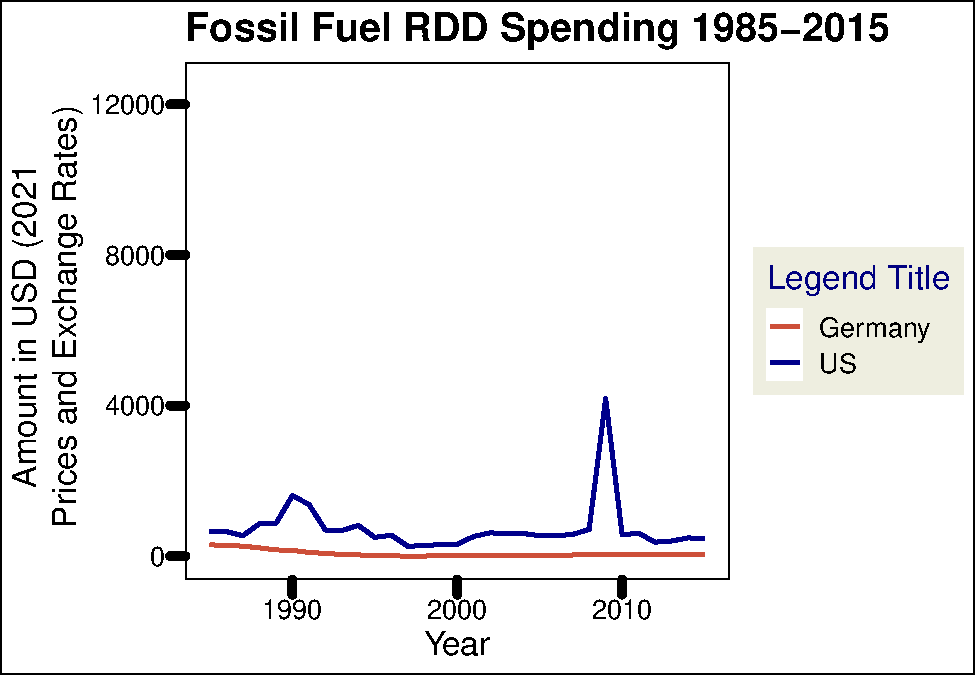
\includegraphics{Chang_Jenkins_Mullens_ENV872_Final_files/figure-latex/Fossil Fuel Germ and US Line-1.pdf}
\caption{US and Germany Fossil Fuel RDD Spending 1985 to 2015. Line
graph used to visualize potential trends.}
\end{figure}

\begin{Shaded}
\begin{Highlighting}[]
\CommentTok{\# Create the US and Germ fossil fuel bar plot}
\NormalTok{US.Germ.Fossil.fuel.Bar.plot }\OtherTok{\textless{}{-}} \FunctionTok{ggplot}\NormalTok{(US.and.Germany.RDD, }\FunctionTok{aes}\NormalTok{(}\AttributeTok{x =}\NormalTok{ Year, }\AttributeTok{y=}\NormalTok{ Fossil.Fuel, }\AttributeTok{fill=}\NormalTok{ Country)) }\SpecialCharTok{+}
  \FunctionTok{geom\_bar}\NormalTok{(}\AttributeTok{stat=} \StringTok{"identity"}\NormalTok{, }\AttributeTok{position =} \StringTok{"stack"}\NormalTok{) }\SpecialCharTok{+}
  \FunctionTok{geom\_bar}\NormalTok{(}\AttributeTok{stat=} \StringTok{"identity"}\NormalTok{, }\AttributeTok{position =} \StringTok{"stack"}\NormalTok{) }\SpecialCharTok{+}
  \FunctionTok{scale\_fill\_manual}\NormalTok{(}\AttributeTok{values =} \FunctionTok{c}\NormalTok{(}\StringTok{"tomato3"}\NormalTok{, }\StringTok{"darkblue"}\NormalTok{)) }\SpecialCharTok{+}
  \FunctionTok{ylim}\NormalTok{(}\DecValTok{0}\NormalTok{, }\DecValTok{5000}\NormalTok{) }\SpecialCharTok{+}
  \FunctionTok{labs}\NormalTok{(}\AttributeTok{fill =} \StringTok{"Country"}\NormalTok{)}\SpecialCharTok{+}
  \FunctionTok{theme}\NormalTok{(}\AttributeTok{axis.text.x =} \FunctionTok{element\_text}\NormalTok{(}\AttributeTok{angle =} \DecValTok{90}\NormalTok{, }\AttributeTok{vjust =} \FloatTok{0.5}\NormalTok{, }\AttributeTok{hjust=}\DecValTok{1}\NormalTok{, }\AttributeTok{size =} \DecValTok{9}\NormalTok{)) }\SpecialCharTok{+}
  \FunctionTok{labs}\NormalTok{(}\AttributeTok{title =} \StringTok{"Fossil Fuel of RDD Spending"}\NormalTok{,}
       \AttributeTok{y=}\StringTok{"Amount in USD (2021 }\SpecialCharTok{\textbackslash{}n}\StringTok{ Prices and Exchange Rates)"}\NormalTok{,}
       \AttributeTok{x=}\StringTok{"Year"}\NormalTok{)}
\FunctionTok{print}\NormalTok{(US.Germ.Fossil.fuel.Bar.plot)}
\end{Highlighting}
\end{Shaded}

\begin{figure}
\centering
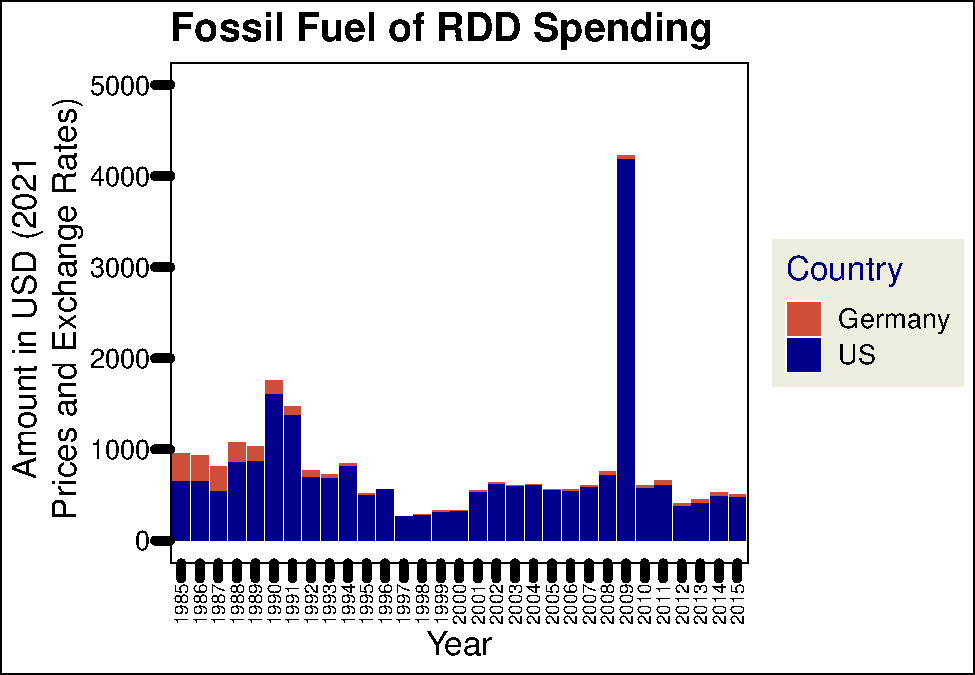
\includegraphics{Chang_Jenkins_Mullens_ENV872_Final_files/figure-latex/US and Germ fossil fuel Bar-1.pdf}
\caption{US and Germany Fossil Fuel RDD Spending 1985 to 2015. Bar graph
used to visually compare relative magnitude of total spending.}
\end{figure}

\begin{Shaded}
\begin{Highlighting}[]
\CommentTok{\#Low Carbon Germ and US Line Plot}
\NormalTok{US.Germ.lowC.plot }\OtherTok{\textless{}{-}} \FunctionTok{ggplot}\NormalTok{(US.and.Germany.RDD,}
                              \FunctionTok{aes}\NormalTok{(}\AttributeTok{x =}\NormalTok{ Date,}
                                  \AttributeTok{y =}\NormalTok{ Low.Carbon.Energy, }
                                  \AttributeTok{color =}\NormalTok{ Country)) }\SpecialCharTok{+} 
  \FunctionTok{geom\_line}\NormalTok{(}\AttributeTok{size=} \FloatTok{0.9}\NormalTok{) }\SpecialCharTok{+}
  \FunctionTok{ylim}\NormalTok{(}\DecValTok{0}\NormalTok{, }\DecValTok{12500}\NormalTok{) }\SpecialCharTok{+}
  \FunctionTok{scale\_color\_manual}\NormalTok{(}\AttributeTok{values =} \FunctionTok{c}\NormalTok{(}\StringTok{"tomato3"}\NormalTok{, }\StringTok{"darkblue"}\NormalTok{)) }\SpecialCharTok{+}
  \FunctionTok{labs}\NormalTok{(}\AttributeTok{title =} \StringTok{"Low Carbon RDD Spending 1985{-}2015"}\NormalTok{,}
       \AttributeTok{y=}\StringTok{"Amount in USD (2021 }\SpecialCharTok{\textbackslash{}n}\StringTok{ Prices and Exchange Rates)"}\NormalTok{,}
       \AttributeTok{x=}\StringTok{"Year"}\NormalTok{,}
       \AttributeTok{color=} \StringTok{"Legend Title"}\NormalTok{)}

\FunctionTok{print}\NormalTok{(US.Germ.lowC.plot)}
\end{Highlighting}
\end{Shaded}

\begin{figure}
\centering
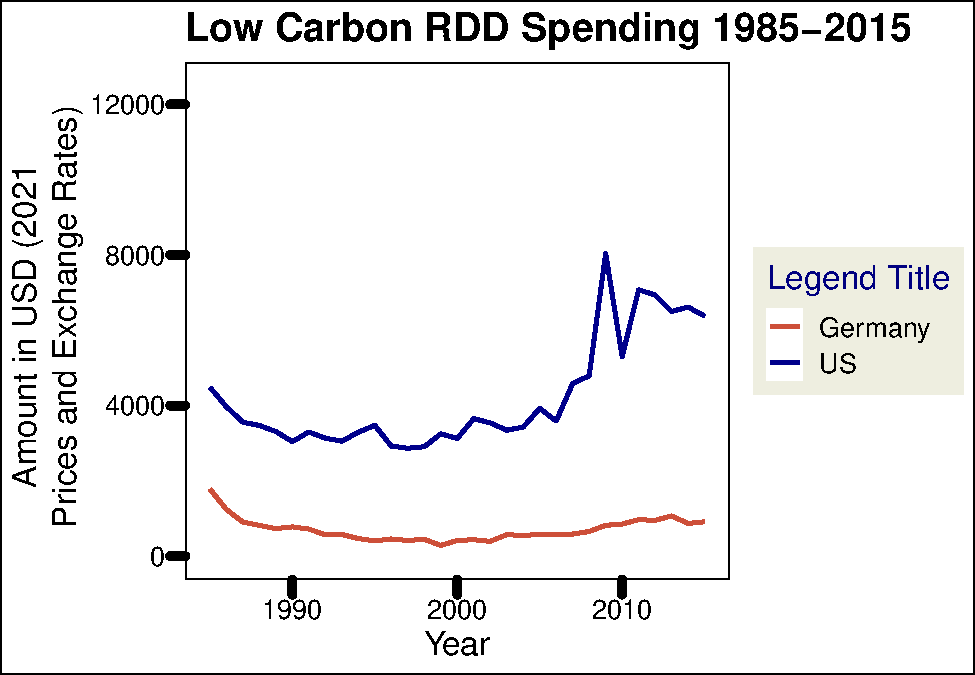
\includegraphics{Chang_Jenkins_Mullens_ENV872_Final_files/figure-latex/Low Carbon Germ and US Line Plot-1.pdf}
\caption{US and Germany Low Carbon Spending 1985 to 2015. Line graph
used to visualize potential trends.}
\end{figure}

\begin{Shaded}
\begin{Highlighting}[]
\CommentTok{\# Create the US and Germ Low Carbon bar plot}
\NormalTok{US.Germ.low.carbon.Bar.plot }\OtherTok{\textless{}{-}} \FunctionTok{ggplot}\NormalTok{(US.and.Germany.RDD, }\FunctionTok{aes}\NormalTok{(}\AttributeTok{x =}\NormalTok{ Year, }\AttributeTok{y=}\NormalTok{ Low.Carbon.Energy, }\AttributeTok{fill=}\NormalTok{ Country)) }\SpecialCharTok{+}
  \FunctionTok{geom\_bar}\NormalTok{(}\AttributeTok{stat=} \StringTok{"identity"}\NormalTok{, }\AttributeTok{position =} \StringTok{"stack"}\NormalTok{) }\SpecialCharTok{+}
  \FunctionTok{geom\_bar}\NormalTok{(}\AttributeTok{stat=} \StringTok{"identity"}\NormalTok{, }\AttributeTok{position =} \StringTok{"stack"}\NormalTok{) }\SpecialCharTok{+}
  \FunctionTok{scale\_fill\_manual}\NormalTok{(}\AttributeTok{values =} \FunctionTok{c}\NormalTok{(}\StringTok{"tomato3"}\NormalTok{, }\StringTok{"darkblue"}\NormalTok{)) }\SpecialCharTok{+}
  \FunctionTok{ylim}\NormalTok{(}\DecValTok{0}\NormalTok{, }\DecValTok{11000}\NormalTok{) }\SpecialCharTok{+}
  \FunctionTok{labs}\NormalTok{(}\AttributeTok{fill =} \StringTok{"Country"}\NormalTok{)}\SpecialCharTok{+}
  \FunctionTok{theme}\NormalTok{(}\AttributeTok{axis.text.x =} \FunctionTok{element\_text}\NormalTok{(}\AttributeTok{angle =} \DecValTok{90}\NormalTok{, }\AttributeTok{vjust =} \FloatTok{0.5}\NormalTok{, }\AttributeTok{hjust=}\DecValTok{1}\NormalTok{, }\AttributeTok{size =} \DecValTok{9}\NormalTok{)) }\SpecialCharTok{+}
  \FunctionTok{labs}\NormalTok{(}\AttributeTok{title =} \StringTok{"Low Carbon RDD Spending 1985{-}2015"}\NormalTok{,}
       \AttributeTok{y=}\StringTok{"Amount in USD (2021 }\SpecialCharTok{\textbackslash{}n}\StringTok{ Prices and Exchange Rates)"}\NormalTok{,}
       \AttributeTok{x=}\StringTok{"Year"}\NormalTok{)}
\FunctionTok{print}\NormalTok{(US.Germ.low.carbon.Bar.plot)}
\end{Highlighting}
\end{Shaded}

\begin{figure}
\centering
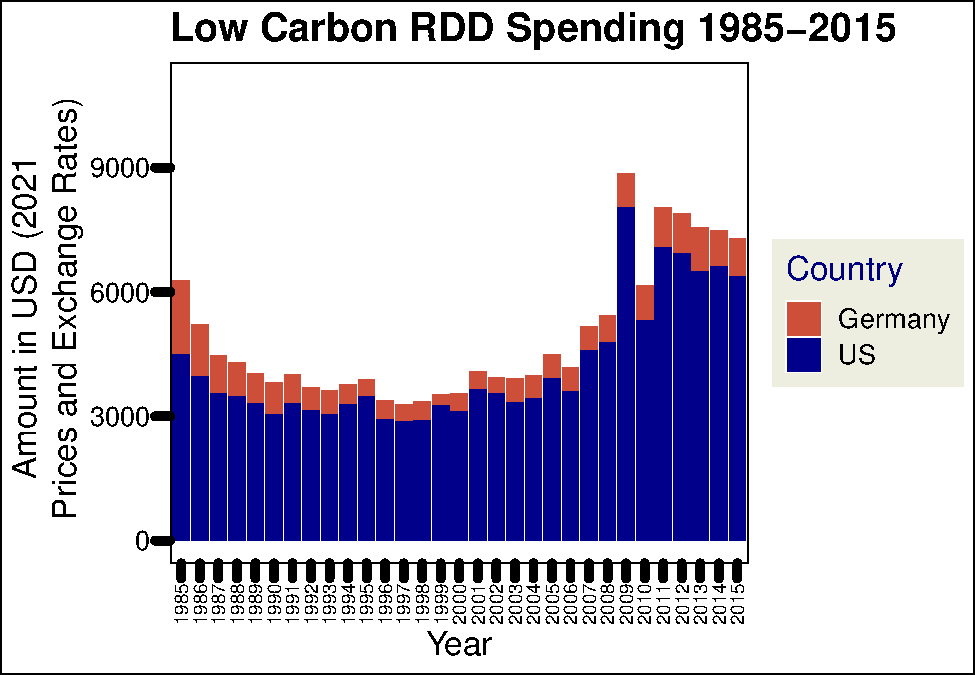
\includegraphics{Chang_Jenkins_Mullens_ENV872_Final_files/figure-latex/US and Germ Low Carbon-1.pdf}
\caption{US and Germany Low Carbon RDD Spending 1985 to 2015, Bar graph
used to visually compare relative magnitude of total spending.}
\end{figure}

\newpage

\hypertarget{analysis}{%
\section{Analysis}\label{analysis}}

Our analysis of this dataset focuses on comparing the mean investment
YoY difference of the Pre-Obama era and the mean investment YoY
difference of the Obama era. However, we need to ensure any changes in
investment is unique to the Obama administration and not occurring
globally. Therefore, we will also utilize t-tests to compare US
investments to Germany's within the same time period.

\begin{Shaded}
\begin{Highlighting}[]
\CommentTok{\#plotting the pre{-}Obama data}
\NormalTok{RDD.US.Eras.plot }\OtherTok{\textless{}{-}}\NormalTok{ RDD.US.Eras }\SpecialCharTok{\%\textgreater{}\%}
  \FunctionTok{ggplot}\NormalTok{(}
         \FunctionTok{aes}\NormalTok{(}\AttributeTok{x=}\NormalTok{ Date,}
             \AttributeTok{y=}\NormalTok{ Percent.Change,}
             \AttributeTok{color=}\NormalTok{ Era)) }\SpecialCharTok{+} 
  \FunctionTok{geom\_line}\NormalTok{() }\SpecialCharTok{+}
  \FunctionTok{geom\_point}\NormalTok{() }\SpecialCharTok{+}
  \FunctionTok{geom\_smooth}\NormalTok{(}\AttributeTok{data =} \FunctionTok{subset}\NormalTok{(RDD.US.Eras, Era }\SpecialCharTok{==} \StringTok{"Pre"}\NormalTok{), }\AttributeTok{method =} \StringTok{"lm"}\NormalTok{, }\AttributeTok{se=}\ConstantTok{FALSE}\NormalTok{, }\AttributeTok{color=} \StringTok{"darkolivegreen4"}\NormalTok{) }\SpecialCharTok{+}
  \FunctionTok{geom\_smooth}\NormalTok{(}\AttributeTok{data =} \FunctionTok{subset}\NormalTok{(RDD.US.Eras, Era }\SpecialCharTok{==} \StringTok{"Obama"}\NormalTok{), }\AttributeTok{method =} \StringTok{"lm"}\NormalTok{, }\AttributeTok{se=}\ConstantTok{FALSE}\NormalTok{, }\AttributeTok{color=} \StringTok{"dodgerblue3"}\NormalTok{) }\SpecialCharTok{+}
  \FunctionTok{labs}\NormalTok{(}\AttributeTok{title =} \StringTok{"Year{-}over{-}Year Percent Change in Public }\SpecialCharTok{\textbackslash{}n}\StringTok{ Low{-}Carbon Energy RD\&D }\SpecialCharTok{\textbackslash{}n}\StringTok{ Spending: U.S."}\NormalTok{,}
       \AttributeTok{y=}\StringTok{"YoY Percent Change"}\NormalTok{,}
       \AttributeTok{x=}\StringTok{"Year"}\NormalTok{) }\SpecialCharTok{+} 
  \FunctionTok{scale\_color\_manual}\NormalTok{(}\AttributeTok{values =} \FunctionTok{c}\NormalTok{(}\StringTok{"darkblue"}\NormalTok{, }\StringTok{"darkgreen"}\NormalTok{)) }\SpecialCharTok{+}
  \FunctionTok{scale\_x\_date}\NormalTok{(}\AttributeTok{date\_breaks =} \StringTok{"2 years"}\NormalTok{, }\AttributeTok{date\_labels =} \StringTok{"\%Y"}\NormalTok{) }\SpecialCharTok{+}
\NormalTok{  our\_theme }\SpecialCharTok{+}
  \FunctionTok{theme}\NormalTok{(}\AttributeTok{axis.text.x =} \FunctionTok{element\_text}\NormalTok{(}\AttributeTok{angle =} \DecValTok{90}\NormalTok{, }\AttributeTok{vjust =} \FloatTok{0.5}\NormalTok{, }\AttributeTok{hjust=}\DecValTok{1}\NormalTok{))}
  
\FunctionTok{print}\NormalTok{(RDD.US.Eras.plot)}
\end{Highlighting}
\end{Shaded}

\begin{verbatim}
## `geom_smooth()` using formula = 'y ~ x'
\end{verbatim}

\begin{verbatim}
## Warning: Removed 1 rows containing non-finite values (`stat_smooth()`).
\end{verbatim}

\begin{verbatim}
## `geom_smooth()` using formula = 'y ~ x'
\end{verbatim}

\begin{verbatim}
## Warning: Removed 1 row containing missing values (`geom_line()`).
\end{verbatim}

\begin{verbatim}
## Warning: Removed 1 rows containing missing values (`geom_point()`).
\end{verbatim}

\begin{figure}
\centering
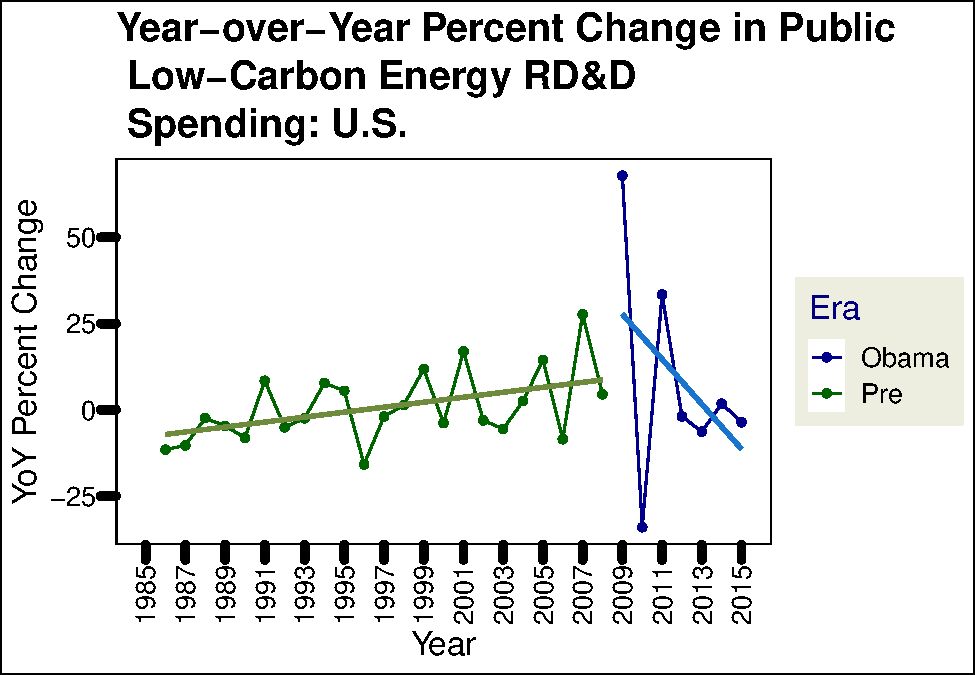
\includegraphics{Chang_Jenkins_Mullens_ENV872_Final_files/figure-latex/visualizing the US data-1.pdf}
\caption{US Year over Year RDD Spending 1985 to 2015}
\end{figure}

\begin{Shaded}
\begin{Highlighting}[]
\CommentTok{\#plotting the data}
\NormalTok{US.Germany.RDD.plot }\OtherTok{\textless{}{-}} \FunctionTok{ggplot}\NormalTok{(US.and.Germany.RDD,}
                              \FunctionTok{aes}\NormalTok{(}\AttributeTok{x =}\NormalTok{ Date,}
                                  \AttributeTok{y =}\NormalTok{ Percent.Change, }
                                  \AttributeTok{color =}\NormalTok{ Country)) }\SpecialCharTok{+} 
  \FunctionTok{geom\_line}\NormalTok{() }\SpecialCharTok{+}
  \FunctionTok{geom\_point}\NormalTok{() }\SpecialCharTok{+}
  \FunctionTok{geom\_smooth}\NormalTok{(}\AttributeTok{data =} \FunctionTok{subset}\NormalTok{(US.and.Germany.RDD, Country }\SpecialCharTok{==} \StringTok{"Germany"}\NormalTok{), }\AttributeTok{method =} \StringTok{"lm"}\NormalTok{, }\AttributeTok{se=}\ConstantTok{FALSE}\NormalTok{, }\AttributeTok{color=} \StringTok{"tomato2"}\NormalTok{) }\SpecialCharTok{+}
  \FunctionTok{geom\_smooth}\NormalTok{(}\AttributeTok{data =} \FunctionTok{subset}\NormalTok{(RDD.US.Eras, Country }\SpecialCharTok{==} \StringTok{"US"}\NormalTok{), }\AttributeTok{method =} \StringTok{"lm"}\NormalTok{, }\AttributeTok{se=}\ConstantTok{FALSE}\NormalTok{, }\AttributeTok{color=} \StringTok{"dodgerblue3"}\NormalTok{) }\SpecialCharTok{+}
  \FunctionTok{scale\_color\_manual}\NormalTok{(}\AttributeTok{values =} \FunctionTok{c}\NormalTok{(}\StringTok{"tomato3"}\NormalTok{, }\StringTok{"darkblue"}\NormalTok{)) }\SpecialCharTok{+}
  \FunctionTok{labs}\NormalTok{(}\AttributeTok{title =} \StringTok{"YoY Change in Public Low{-}Carbon }\SpecialCharTok{\textbackslash{}n}\StringTok{ Energy RD\&D Spending: }\SpecialCharTok{\textbackslash{}n}\StringTok{ US vs. Germany"}\NormalTok{,}
       \AttributeTok{y=}\StringTok{"Year{-}over{-}Year Percent Change"}\NormalTok{,}
       \AttributeTok{x=}\StringTok{"Year"}\NormalTok{) }\SpecialCharTok{+} 
  \FunctionTok{scale\_x\_date}\NormalTok{(}\AttributeTok{date\_breaks =} \StringTok{"2 years"}\NormalTok{, }\AttributeTok{date\_labels =} \StringTok{"\%Y"}\NormalTok{) }\SpecialCharTok{+}
\NormalTok{  our\_theme }\SpecialCharTok{+}
  \FunctionTok{theme}\NormalTok{(}\AttributeTok{axis.text.x =} \FunctionTok{element\_text}\NormalTok{(}\AttributeTok{angle =} \DecValTok{90}\NormalTok{, }\AttributeTok{vjust =} \FloatTok{0.5}\NormalTok{, }\AttributeTok{hjust=}\DecValTok{1}\NormalTok{))}
  
\FunctionTok{print}\NormalTok{(US.Germany.RDD.plot)}
\end{Highlighting}
\end{Shaded}

\begin{verbatim}
## `geom_smooth()` using formula = 'y ~ x'
\end{verbatim}

\begin{verbatim}
## Warning: Removed 1 rows containing non-finite values (`stat_smooth()`).
\end{verbatim}

\begin{verbatim}
## `geom_smooth()` using formula = 'y ~ x'
\end{verbatim}

\begin{verbatim}
## Warning: Removed 1 rows containing non-finite values (`stat_smooth()`).
\end{verbatim}

\begin{verbatim}
## Warning: Removed 2 rows containing missing values (`geom_line()`).
\end{verbatim}

\begin{verbatim}
## Warning: Removed 2 rows containing missing values (`geom_point()`).
\end{verbatim}

\begin{figure}
\centering
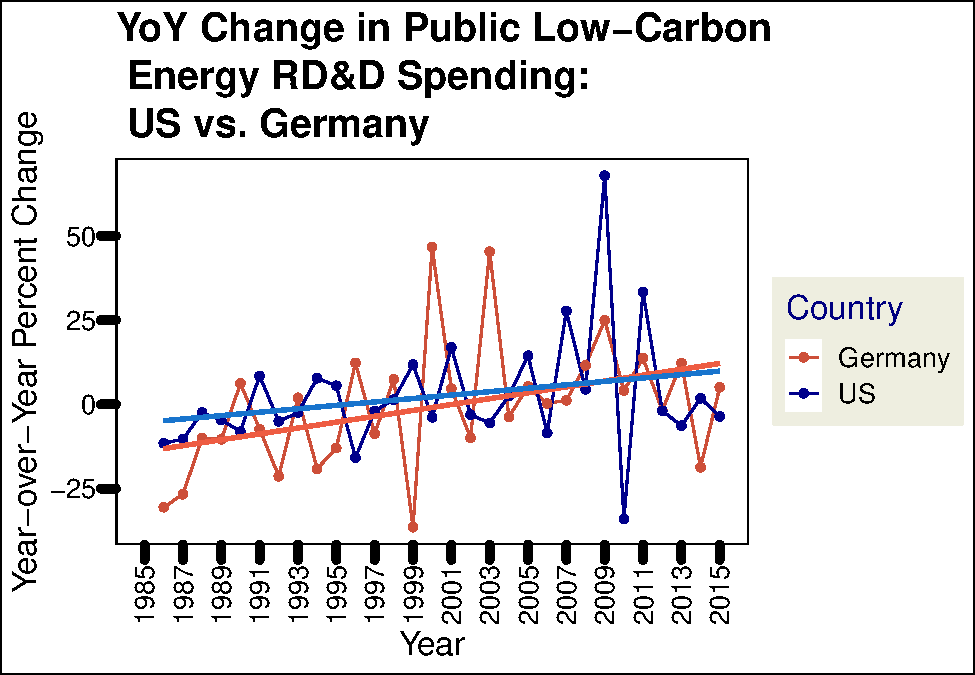
\includegraphics{Chang_Jenkins_Mullens_ENV872_Final_files/figure-latex/visualizing the US and Germany data together-1.pdf}
\caption{US and Germany Year over Year RDD Spending 1985 to 2015}
\end{figure}

\begin{Shaded}
\begin{Highlighting}[]
\CommentTok{\#plotting the data}
\NormalTok{US.Germany.RDD.pre.plot }\OtherTok{\textless{}{-}}\NormalTok{ US.and.Germany.RDD }\SpecialCharTok{\%\textgreater{}\%}
  \FunctionTok{filter}\NormalTok{(Era }\SpecialCharTok{==} \StringTok{"Pre"}\NormalTok{) }\SpecialCharTok{\%\textgreater{}\%}
  \FunctionTok{ggplot}\NormalTok{(}\FunctionTok{aes}\NormalTok{(}\AttributeTok{x =}\NormalTok{ Date,}
             \AttributeTok{y =}\NormalTok{ Percent.Change, }
             \AttributeTok{color =}\NormalTok{ Country)) }\SpecialCharTok{+} 
  \FunctionTok{geom\_line}\NormalTok{() }\SpecialCharTok{+}
  \FunctionTok{geom\_point}\NormalTok{() }\SpecialCharTok{+}
  \FunctionTok{geom\_smooth}\NormalTok{(}\AttributeTok{data =} \FunctionTok{subset}\NormalTok{(US.and.Germany.RDD, Country }\SpecialCharTok{==} \StringTok{"Germany"} \SpecialCharTok{\&}\NormalTok{ Era }\SpecialCharTok{==} \StringTok{"Pre"}\NormalTok{), }\AttributeTok{method =} \StringTok{"lm"}\NormalTok{, }\AttributeTok{se=}\ConstantTok{FALSE}\NormalTok{, }\AttributeTok{color=} \StringTok{"tomato2"}\NormalTok{) }\SpecialCharTok{+}
  \FunctionTok{geom\_smooth}\NormalTok{(}\AttributeTok{data =} \FunctionTok{subset}\NormalTok{(RDD.US.Eras, Country }\SpecialCharTok{==} \StringTok{"US"} \SpecialCharTok{\&}\NormalTok{ Era }\SpecialCharTok{==} \StringTok{"Pre"}\NormalTok{), }\AttributeTok{method =} \StringTok{"lm"}\NormalTok{, }\AttributeTok{se=}\ConstantTok{FALSE}\NormalTok{, }\AttributeTok{color=} \StringTok{"blue3"}\NormalTok{) }\SpecialCharTok{+}
  \FunctionTok{scale\_color\_manual}\NormalTok{(}\AttributeTok{values =} \FunctionTok{c}\NormalTok{(}\StringTok{"tomato3"}\NormalTok{, }\StringTok{"darkblue"}\NormalTok{)) }\SpecialCharTok{+}
  \FunctionTok{labs}\NormalTok{(}\AttributeTok{title =} \StringTok{"YoY Change in Public Low{-}Carbon }\SpecialCharTok{\textbackslash{}n}\StringTok{ Energy RD\&D Spending: }\SpecialCharTok{\textbackslash{}n}\StringTok{ US vs. Germany"}\NormalTok{,}
       \AttributeTok{y=}\StringTok{"Year{-}over{-}Year Percent Change"}\NormalTok{,}
       \AttributeTok{x=}\StringTok{"Year"}\NormalTok{) }\SpecialCharTok{+} 
  \FunctionTok{scale\_x\_date}\NormalTok{(}\AttributeTok{date\_breaks =} \StringTok{"1 years"}\NormalTok{, }\AttributeTok{date\_labels =} \StringTok{"\%Y"}\NormalTok{) }\SpecialCharTok{+}
\NormalTok{  our\_theme }\SpecialCharTok{+}
  \FunctionTok{theme}\NormalTok{(}\AttributeTok{axis.text.x =} \FunctionTok{element\_text}\NormalTok{(}\AttributeTok{angle =} \DecValTok{90}\NormalTok{, }\AttributeTok{vjust =} \FloatTok{0.5}\NormalTok{, }\AttributeTok{hjust=}\DecValTok{1}\NormalTok{, }\AttributeTok{size=}\DecValTok{9}\NormalTok{))}
  
\FunctionTok{print}\NormalTok{(US.Germany.RDD.pre.plot)}
\end{Highlighting}
\end{Shaded}

\begin{verbatim}
## `geom_smooth()` using formula = 'y ~ x'
\end{verbatim}

\begin{verbatim}
## Warning: Removed 1 rows containing non-finite values (`stat_smooth()`).
\end{verbatim}

\begin{verbatim}
## `geom_smooth()` using formula = 'y ~ x'
\end{verbatim}

\begin{verbatim}
## Warning: Removed 1 rows containing non-finite values (`stat_smooth()`).
\end{verbatim}

\begin{verbatim}
## Warning: Removed 2 rows containing missing values (`geom_line()`).
\end{verbatim}

\begin{verbatim}
## Warning: Removed 2 rows containing missing values (`geom_point()`).
\end{verbatim}

\begin{figure}
\centering
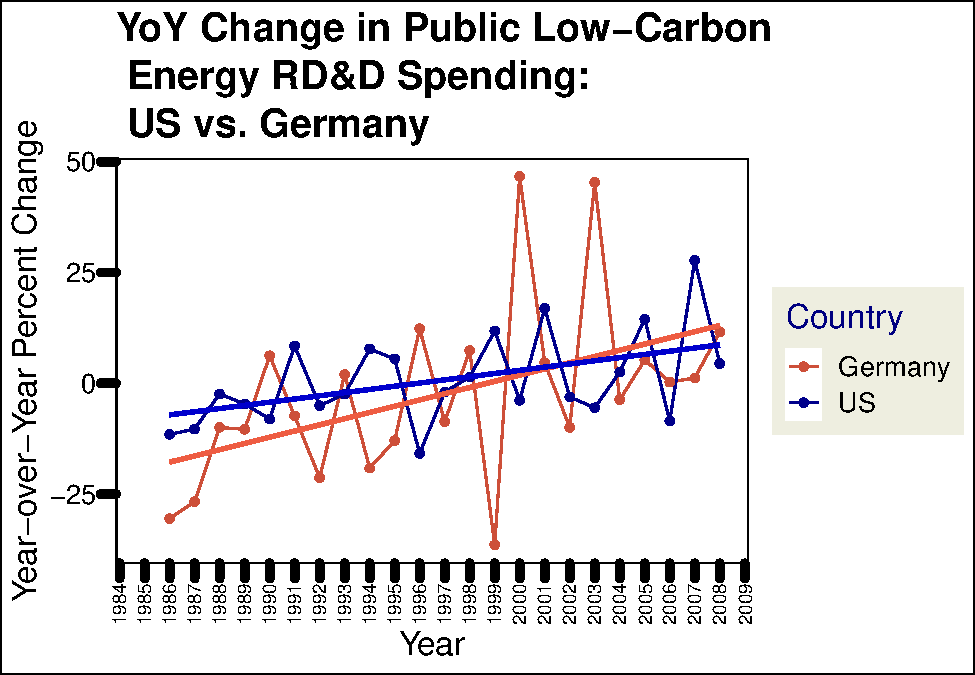
\includegraphics{Chang_Jenkins_Mullens_ENV872_Final_files/figure-latex/visualizing the pre US and Germany data together-1.pdf}
\caption{US and Germany Year over Year RDD Spending 1985 to 2008}
\end{figure}

\begin{Shaded}
\begin{Highlighting}[]
\CommentTok{\#plotting the data}
\NormalTok{US.Germany.RDD.Obama.plot }\OtherTok{\textless{}{-}}\NormalTok{ US.and.Germany.RDD }\SpecialCharTok{\%\textgreater{}\%}
  \FunctionTok{filter}\NormalTok{(Era }\SpecialCharTok{==} \StringTok{"Obama"}\NormalTok{) }\SpecialCharTok{\%\textgreater{}\%}
  \FunctionTok{ggplot}\NormalTok{(}\FunctionTok{aes}\NormalTok{(}\AttributeTok{x =}\NormalTok{ Date,}
             \AttributeTok{y =}\NormalTok{ Percent.Change, }
             \AttributeTok{color =}\NormalTok{ Country)) }\SpecialCharTok{+} 
  \FunctionTok{geom\_line}\NormalTok{() }\SpecialCharTok{+}
  \FunctionTok{geom\_point}\NormalTok{() }\SpecialCharTok{+}
  \FunctionTok{geom\_smooth}\NormalTok{(}\AttributeTok{data =} \FunctionTok{subset}\NormalTok{(US.and.Germany.RDD, Country }\SpecialCharTok{==} \StringTok{"Germany"} \SpecialCharTok{\&}\NormalTok{ Era }\SpecialCharTok{==} \StringTok{"Obama"}\NormalTok{), }\AttributeTok{method =} \StringTok{"lm"}\NormalTok{, }\AttributeTok{se=}\ConstantTok{FALSE}\NormalTok{, }\AttributeTok{color=} \StringTok{"tomato2"}\NormalTok{) }\SpecialCharTok{+}
  \FunctionTok{geom\_smooth}\NormalTok{(}\AttributeTok{data =} \FunctionTok{subset}\NormalTok{(RDD.US.Eras, Country }\SpecialCharTok{==} \StringTok{"US"} \SpecialCharTok{\&}\NormalTok{ Era }\SpecialCharTok{==} \StringTok{"Obama"}\NormalTok{), }\AttributeTok{method =} \StringTok{"lm"}\NormalTok{, }\AttributeTok{se=}\ConstantTok{FALSE}\NormalTok{, }\AttributeTok{color=} \StringTok{"blue3"}\NormalTok{) }\SpecialCharTok{+}
  \FunctionTok{scale\_color\_manual}\NormalTok{(}\AttributeTok{values =} \FunctionTok{c}\NormalTok{(}\StringTok{"tomato3"}\NormalTok{, }\StringTok{"darkblue"}\NormalTok{)) }\SpecialCharTok{+}
  \FunctionTok{labs}\NormalTok{(}\AttributeTok{title =} \StringTok{"YoY Change in Public Low{-}Carbon }\SpecialCharTok{\textbackslash{}n}\StringTok{ Energy RD\&D Spending: }\SpecialCharTok{\textbackslash{}n}\StringTok{ US vs. Germany"}\NormalTok{,}
       \AttributeTok{y=}\StringTok{"Year{-}over{-}Year Percent Change"}\NormalTok{,}
       \AttributeTok{x=}\StringTok{"Year"}\NormalTok{) }\SpecialCharTok{+} 
  \FunctionTok{scale\_x\_date}\NormalTok{(}\AttributeTok{date\_breaks =} \StringTok{"1 years"}\NormalTok{, }\AttributeTok{date\_labels =} \StringTok{"\%Y"}\NormalTok{) }\SpecialCharTok{+}
\NormalTok{  our\_theme }\SpecialCharTok{+}
  \FunctionTok{theme}\NormalTok{(}\AttributeTok{axis.text.x =} \FunctionTok{element\_text}\NormalTok{(}\AttributeTok{angle =} \DecValTok{90}\NormalTok{, }\AttributeTok{vjust =} \FloatTok{0.5}\NormalTok{, }\AttributeTok{hjust=}\DecValTok{1}\NormalTok{, }\AttributeTok{size=}\DecValTok{9}\NormalTok{))}
  
\FunctionTok{print}\NormalTok{(US.Germany.RDD.Obama.plot)}
\end{Highlighting}
\end{Shaded}

\begin{verbatim}
## `geom_smooth()` using formula = 'y ~ x'
## `geom_smooth()` using formula = 'y ~ x'
\end{verbatim}

\begin{figure}
\centering
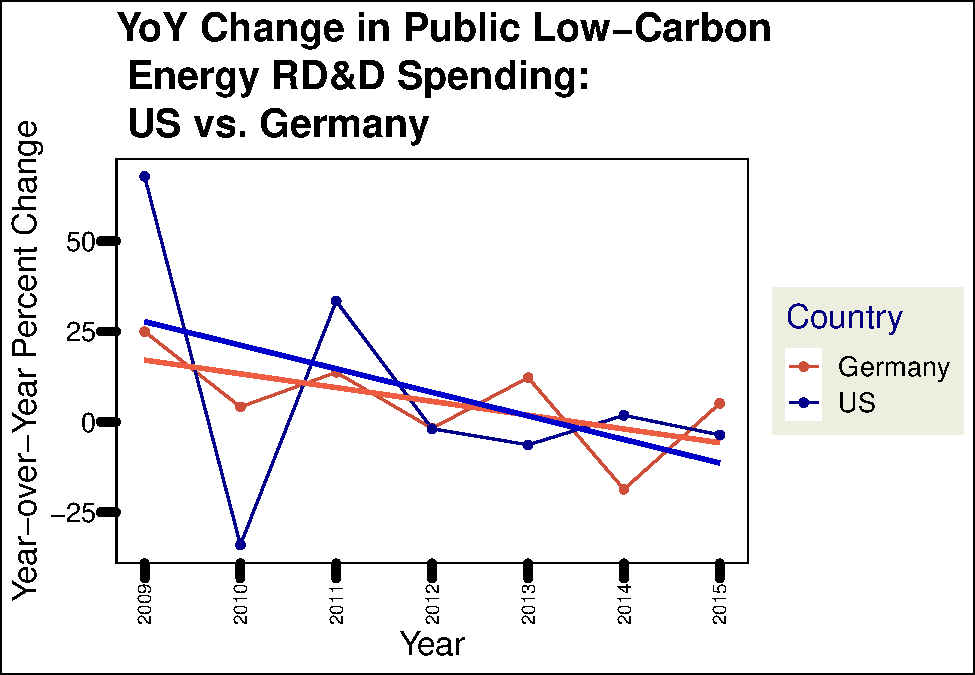
\includegraphics{Chang_Jenkins_Mullens_ENV872_Final_files/figure-latex/visualizing Obama US and Germany data together-1.pdf}
\caption{US and Germany Year over Year RDD Spending 2009 to 2015}
\end{figure}

\begin{Shaded}
\begin{Highlighting}[]
\CommentTok{\# T{-}test \#1) U.S. Public Low{-}Carbon Energy RD\&D Spending: Pre{-}Obama (1985{-}2008) vs. during Obama Administration (2009{-}2015)}

        \CommentTok{\#Alternative hypothesis == YoY change in public spending on lower{-}carbon energy RD\&D is significant during Obama administration}

        \CommentTok{\#Run two{-}sample T{-}test on US RDD "Eras" data to determine if mean YoY change in investment is the same or different before vs. during Obama admin}

\NormalTok{US.Pre.v.Post.Obama.ttest }\OtherTok{\textless{}{-}} \FunctionTok{t.test}\NormalTok{(RDD.US.Eras}\SpecialCharTok{$}\NormalTok{Percent.Change }\SpecialCharTok{\textasciitilde{}} 
\NormalTok{                                      RDD.US.Eras}\SpecialCharTok{$}\NormalTok{Era)}

\NormalTok{US.Pre.v.Post.Obama.ttest}
\end{Highlighting}
\end{Shaded}

\begin{verbatim}
## 
##  Welch Two Sample t-test
## 
## data:  RDD.US.Eras$Percent.Change by RDD.US.Eras$Era
## t = 0.58747, df = 6.3612, p-value = 0.5771
## alternative hypothesis: true difference in means between group Obama and group Pre is not equal to 0
## 95 percent confidence interval:
##  -23.01113  37.81629
## sample estimates:
## mean in group Obama   mean in group Pre 
##           8.1695963           0.7670191
\end{verbatim}

\begin{Shaded}
\begin{Highlighting}[]
         \CommentTok{\#The p{-}value is 0.5771 which is greater than 0.05 so we must accept our null hypothesis. Therefore, mean year{-}over{-}year change in public low{-}carbon RD\&D spending during the Obama presidency (2009{-}2015) was not statistically distinct from the Pre{-}Obama era (1985{-}2008) YoY spending change.}

\CommentTok{\#{-}{-}{-}{-}{-}{-}{-}{-}{-}{-}{-}{-}{-}{-}{-}{-}{-}{-}{-}{-}{-}{-}{-}{-}{-}{-}{-}}
  
\CommentTok{\# T{-}test \#2) Pre{-}Obama Public Low{-}Carbon RD\&D Spending (1985{-}2008): U.S. vs Germany }

         \CommentTok{\#Alternative hypothesis == Prior to Obama\textquotesingle{}s inauguration (in the period spanning 1985{-}2008), the mean YoY change in public low{-}carbon RDD spending in the United States is not statistically distinct from Germany\textquotesingle{}s mean YoY change in public spending   }
    
          \DocumentationTok{\#\#\^{} this hypothesis would mean that our null hypothesis is: prior to obama admin, the mean YoY change in public low{-}carbon RDD spending in the United States IS statistically distinct from germany  }

\NormalTok{Pre.}\FloatTok{2009.}\NormalTok{US.Germany.RDD }\OtherTok{\textless{}{-}} \FunctionTok{filter}\NormalTok{(US.and.Germany.RDD, Year }\SpecialCharTok{\%in\%} \FunctionTok{c}\NormalTok{(}\DecValTok{1985}\SpecialCharTok{:}\DecValTok{2008}\NormalTok{))}
  
\NormalTok{Pre.}\FloatTok{2009.}\NormalTok{US.Germany.ttest }\OtherTok{\textless{}{-}} \FunctionTok{t.test}\NormalTok{(Pre.}\FloatTok{2009.}\NormalTok{US.Germany.RDD}\SpecialCharTok{$}\NormalTok{Percent.Change }\SpecialCharTok{\textasciitilde{}} 
\NormalTok{                                      Pre.}\FloatTok{2009.}\NormalTok{US.Germany.RDD}\SpecialCharTok{$}\NormalTok{Country)}

\NormalTok{Pre.}\FloatTok{2009.}\NormalTok{US.Germany.ttest}
\end{Highlighting}
\end{Shaded}

\begin{verbatim}
## 
##  Welch Two Sample t-test
## 
## data:  Pre.2009.US.Germany.RDD$Percent.Change by Pre.2009.US.Germany.RDD$Country
## t = -0.66411, df = 32.7, p-value = 0.5113
## alternative hypothesis: true difference in means between group Germany and group US is not equal to 0
## 95 percent confidence interval:
##  -12.743123   6.472836
## sample estimates:
## mean in group Germany      mean in group US 
##            -2.3681247             0.7670191
\end{verbatim}

\begin{Shaded}
\begin{Highlighting}[]
      \CommentTok{\#The p{-}value is 0.5113 which is greater than 0.05 so we must accept our null hypothesis. Therefore, in the period prior to Obama\textquotesingle{}s presidency (1985{-}2008), the mean year{-}over{-}year change in public low{-}carbon RD\&D spending in the U.S. was statistically distinct from Germany.}
    
      \CommentTok{\#NOTES FROM GOOGLE RE: NULL: If the p{-}value is below your threshold of significance (typically p \textless{} 0.05), then you can reject the null hypothesis, but this does not necessarily mean that your alternative hypothesis is true.}

\CommentTok{\#{-}{-}{-}{-}{-}{-}{-}{-}{-}{-}{-}{-}{-}{-}{-}{-}{-}{-}{-}{-}{-}{-}{-}{-}{-}{-}{-}{-}{-}{-}}
  
\CommentTok{\# T{-}test \#3) Obama{-}era Public Low{-}carbon RD\&D Spending (2009{-}2015): United States vs. Germany}

            \DocumentationTok{\#\#Alternative Hypothesis == during the Obama presidency (2009{-}2015), the mean YoY change in public low{-}carbon RDD spending in the United States was statistically distinct from the mean YoY change in Germany }

\NormalTok{Post.}\FloatTok{2009.}\NormalTok{US.Germany.RDD }\OtherTok{\textless{}{-}} \FunctionTok{filter}\NormalTok{(US.and.Germany.RDD, Year }\SpecialCharTok{\%in\%} \FunctionTok{c}\NormalTok{(}\DecValTok{2009}\SpecialCharTok{:}\DecValTok{2015}\NormalTok{))}
  
\NormalTok{Post.}\FloatTok{2009.}\NormalTok{US.Germany.ttest }\OtherTok{\textless{}{-}} \FunctionTok{t.test}\NormalTok{(Post.}\FloatTok{2009.}\NormalTok{US.Germany.RDD}\SpecialCharTok{$}\NormalTok{Percent.Change }\SpecialCharTok{\textasciitilde{}} 
\NormalTok{                                      Post.}\FloatTok{2009.}\NormalTok{US.Germany.RDD}\SpecialCharTok{$}\NormalTok{Country)}

\NormalTok{Post.}\FloatTok{2009.}\NormalTok{US.Germany.ttest}
\end{Highlighting}
\end{Shaded}

\begin{verbatim}
## 
##  Welch Two Sample t-test
## 
## data:  Post.2009.US.Germany.RDD$Percent.Change by Post.2009.US.Germany.RDD$Country
## t = -0.18605, df = 8.0331, p-value = 0.857
## alternative hypothesis: true difference in means between group Germany and group US is not equal to 0
## 95 percent confidence interval:
##  -33.51499  28.50738
## sample estimates:
## mean in group Germany      mean in group US 
##              5.665790              8.169596
\end{verbatim}

\begin{Shaded}
\begin{Highlighting}[]
          \CommentTok{\#The p{-}value is 0.857 which is greater than 0.05 so the null hypothesis is accepted. Therefore, Obama{-}era (2009{-}2015) mean year{-}over{-}year change in public low{-}carbon RD\&D spending in the U.S. was not statistically distinct from Germany.}
\end{Highlighting}
\end{Shaded}

\newpage

\hypertarget{summary-and-conclusions}{%
\section{Summary and Conclusions}\label{summary-and-conclusions}}

\newpage

\#Scripts, data and code The repository linked at the beginning contains
both the raw data, wrangled data, and code utilized. They are found in
their respective folders.

\#Quality assurance Please note that any conclusions created by this
report are limited as only one source of data and one variable were
utilized. Further examination of additional metrics and countries are
recommended for future analyses.

\newpage

\#Appendix

\begin{Shaded}
\begin{Highlighting}[]
\CommentTok{\# Create the combined bar plot}
\NormalTok{RDD.US.Eras.Bar.plot }\OtherTok{\textless{}{-}} \FunctionTok{ggplot}\NormalTok{(RDD.US.Eras, }\FunctionTok{aes}\NormalTok{(}\AttributeTok{x =}\NormalTok{ Year)) }\SpecialCharTok{+}
  \FunctionTok{geom\_bar}\NormalTok{(}\FunctionTok{aes}\NormalTok{(}\AttributeTok{y =}\NormalTok{ Total.Budget, }\AttributeTok{fill =} \StringTok{"Total.budget"}\NormalTok{), }\AttributeTok{stat=} \StringTok{"identity"}\NormalTok{, }\AttributeTok{position =} \StringTok{"identity"}\NormalTok{) }\SpecialCharTok{+}
  \FunctionTok{geom\_bar}\NormalTok{(}\FunctionTok{aes}\NormalTok{(}\AttributeTok{y =}\NormalTok{ Low.Carbon.Energy, }\AttributeTok{fill =} \StringTok{"Low.Carbon"}\NormalTok{), }\AttributeTok{stat=} \StringTok{"identity"}\NormalTok{, }\AttributeTok{position =} \StringTok{"identity"}\NormalTok{) }\SpecialCharTok{+}
  \FunctionTok{geom\_bar}\NormalTok{(}\FunctionTok{aes}\NormalTok{(}\AttributeTok{y =}\NormalTok{ Fossil.Fuel, }\AttributeTok{fill =} \StringTok{"Fossil.Fuels"}\NormalTok{), }\AttributeTok{stat=} \StringTok{"identity"}\NormalTok{, }\AttributeTok{position =} \StringTok{"identity"}\NormalTok{) }\SpecialCharTok{+}
  \FunctionTok{scale\_fill\_manual}\NormalTok{(}\AttributeTok{values =} \FunctionTok{c}\NormalTok{(}\StringTok{"Fossil.Fuels"} \OtherTok{=} \StringTok{"midnightblue"}\NormalTok{, }\StringTok{"Low.Carbon"} \OtherTok{=} \StringTok{"darkolivegreen3"}\NormalTok{, }\StringTok{"Total.budget"} \OtherTok{=} \StringTok{"sienna3"}\NormalTok{)) }\SpecialCharTok{+}
  \FunctionTok{labs}\NormalTok{(}\AttributeTok{fill =} \StringTok{"Budget Portion"}\NormalTok{)}\SpecialCharTok{+}
  \FunctionTok{theme}\NormalTok{(}\AttributeTok{axis.text.x =} \FunctionTok{element\_text}\NormalTok{(}\AttributeTok{angle =} \DecValTok{90}\NormalTok{, }\AttributeTok{vjust =} \FloatTok{0.5}\NormalTok{, }\AttributeTok{hjust=}\DecValTok{1}\NormalTok{)) }\SpecialCharTok{+}
  \FunctionTok{labs}\NormalTok{(}\AttributeTok{title =} \StringTok{"Proportion of RDD Spending"}\NormalTok{,}
       \AttributeTok{y=}\StringTok{"Amount in USD (2021 }\SpecialCharTok{\textbackslash{}n}\StringTok{ Pricess and Exchange Rates)"}\NormalTok{,}
       \AttributeTok{x=}\StringTok{"Year"}\NormalTok{)}
\FunctionTok{print}\NormalTok{(RDD.US.Eras.Bar.plot)}
\end{Highlighting}
\end{Shaded}

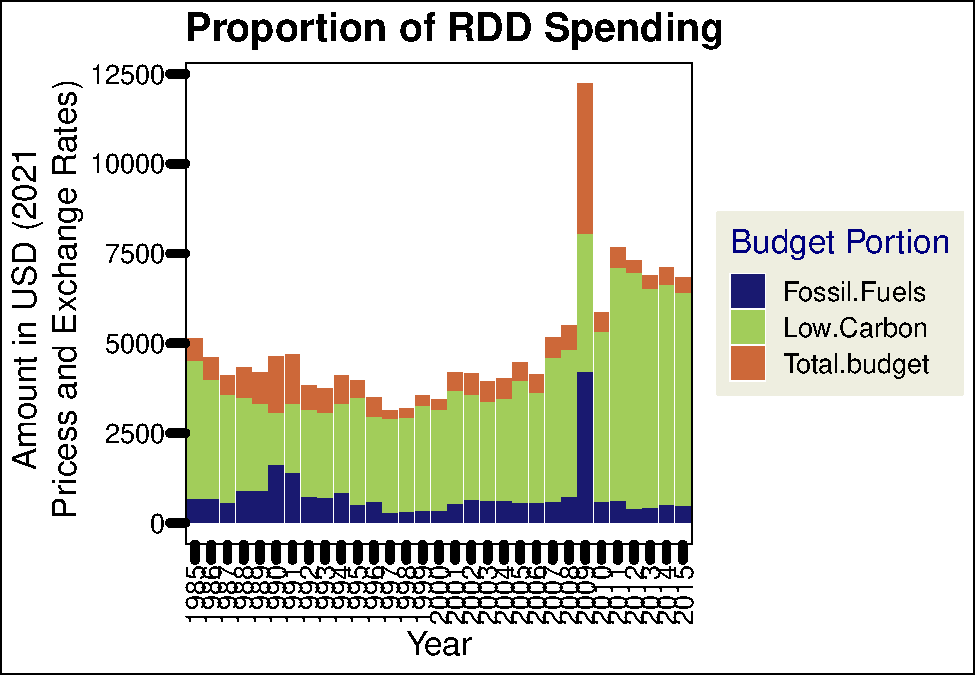
\includegraphics{Chang_Jenkins_Mullens_ENV872_Final_files/figure-latex/Combined bar plot of US RDD-1.pdf}

\hypertarget{references}{%
\section{References}\label{references}}

\textless add references here if relevant, otherwise delete this
section\textgreater{}

\end{document}
